\documentclass[10pt]{article}
\usepackage{siunitx,gensymb} % gensym gives degree
\usepackage{amsmath}
\usepackage{newtxtext,newtxmath}
\usepackage[numbers]{natbib}
\usepackage{graphicx}
\usepackage{xcolor}
\usepackage[bookmarks=true,bookmarksnumbered=true,hidelinks]{hyperref}
\usepackage{cleveref}
\usepackage{algorithm2e}
\usepackage{svg}
\usepackage[compact]{titlesec}
\usepackage[]{acronym} % provides \acronym 
\graphicspath{{../figures/}}

% --- Math ---
\newcommand{\pp}[2]{\frac{\partial #1}{\partial #2}}
\newcommand{\ppt}[2]{\frac{\partial^2 #1}{\partial #2^2}}
\newcommand{\pptt}[2]{\frac{\partial^3 #1}{\partial #2^3}}
\newcommand{\ppttt}[2]{\frac{\partial^4 #1}{\partial #2^4}}
\newcommand{\DD}[2]{\frac{\textrm{D} #1}{\textrm{D} #2}}
\newcommand{\dd}[2]{\frac{\textrm{d} #1}{\textrm{d} #2}}
\newcommand{\ddt}[2]{\frac{d^2 #1}{d #2^2}}
\newcommand{\ddtt}[2]{\frac{d^3 #1}{d #2^3}}
\newcommand{\ddttt}[2]{\frac{d^4 #1}{d #2^4}}
\newcommand{\mbb}[1]{\mathbb{#1}}    % math blackboard
\newcommand{\mbf}[1]{\mathbf{#1}}
\newcommand{\mrm}[1]{\mathrm{#1}}
\newcommand{\mcal}[1]{\mathcal{#1}}  % math calligraphy
\newcommand{\mbfh}[1]{\widehat{\mathbf{#1}}}
\newcommand{\mbfv}[1]{\vec{\mathbf{#1}}}
\newcommand{\half}{\frac{1}{2}}
\newcommand{\third}{\frac{1}{3}}
% --- Equations ---
\newcommand{\be}{\begin{eqnarray}}
\newcommand{\ee}{\end{eqnarray}}
\newcommand{\ben}{\begin{eqnarray*}}
\newcommand{\een}{\end{eqnarray*}}
\newcommand{\beq}{\begin{equation}
    \begin{aligned}
        }
\newcommand{\eeq}{\end{aligned}
\end{equation}
}
% --- Numerical methods ---
\newcommand{\dx}{d\mbf{x}}
\newcommand{\Dt}{\Delta t}
\newcommand{\ih}{\hat{i}}
\newcommand{\jh}{\hat{j}}
\newcommand{\kh}{\hat{k}}
\newcommand{\nh}{\hat{n}}
\newcommand{\xh}{\hat{x}}
\newcommand{\yh}{\hat{y}}
\newcommand{\zh}{\hat{z}}
\newcommand{\uj}[1]{u_{j  #1 }}
\newcommand{\ujn}[2]{u_{j  #1 }^{n  #2}}
\newcommand{\BigO}{\mathcal{O}}
\newcommand{\CFL}{{\mbox{CFL}}}
\newcommand{\opt}[1]{#1 (x^{\star})}
% --- Flow ---
\newcommand{\Uinf}{U_{\infty}}
\newcommand{\Vinf}{V_{\infty}}
\newcommand{\Minf}{M_{\infty}}
\newcommand{\bVinf}{\mbf{V}_{\infty}}
\newcommand{\pinf}{p_{\infty}}
\newcommand{\patm}{p_{\textrm{atm}}}
\newcommand{\cpmin}{C_{p_{\tn{min}}}}
% --- Other Shorthands ---
\newcommand{\tn}[1]{\textnormal{#1}}
\newcommand{\fw} {forward swept\:}
\newcommand{\un} {unswept\:}
\newcommand{\bw} {backward swept\:}
\newcommand{\scriptth}{\scriptsize \textnormal{th}}
\newcommand{\cfrp}[1] {CFRP #1$^\circ$\:}
\newcommand{\tss}[1]{\textsuperscript{#1}}
\newcommand{\wrt} {with respect to\:}

% --- Spacings ---
\setlength{\headsep}{0.0in}
\setlength{\topmargin}{0.0in}
\setlength{\textheight}{8.8in}
\setlength{\textwidth}{6.8in}
\setlength{\oddsidemargin}{-.15in}
\setlength{\evensidemargin}{-.15in}
\setlength{\unitlength}{1in}

\bibliographystyle{unsrtnat}


\begin{document}

\title{\vspace{-1.5cm} DCFoil Developer and User Documentation}
\author{Galen W.~Ng}
\maketitle
% ==============================================================================
%                         BEGIN
% ==============================================================================
\section*{Summary}
% 
DCFoil is a program for the dynamic analysis and design optimization of composite hydrofoils.
\begin{figure}[htbp!]
    \centering
    % reference: trim={<left> <lower> <right> <upper>}
    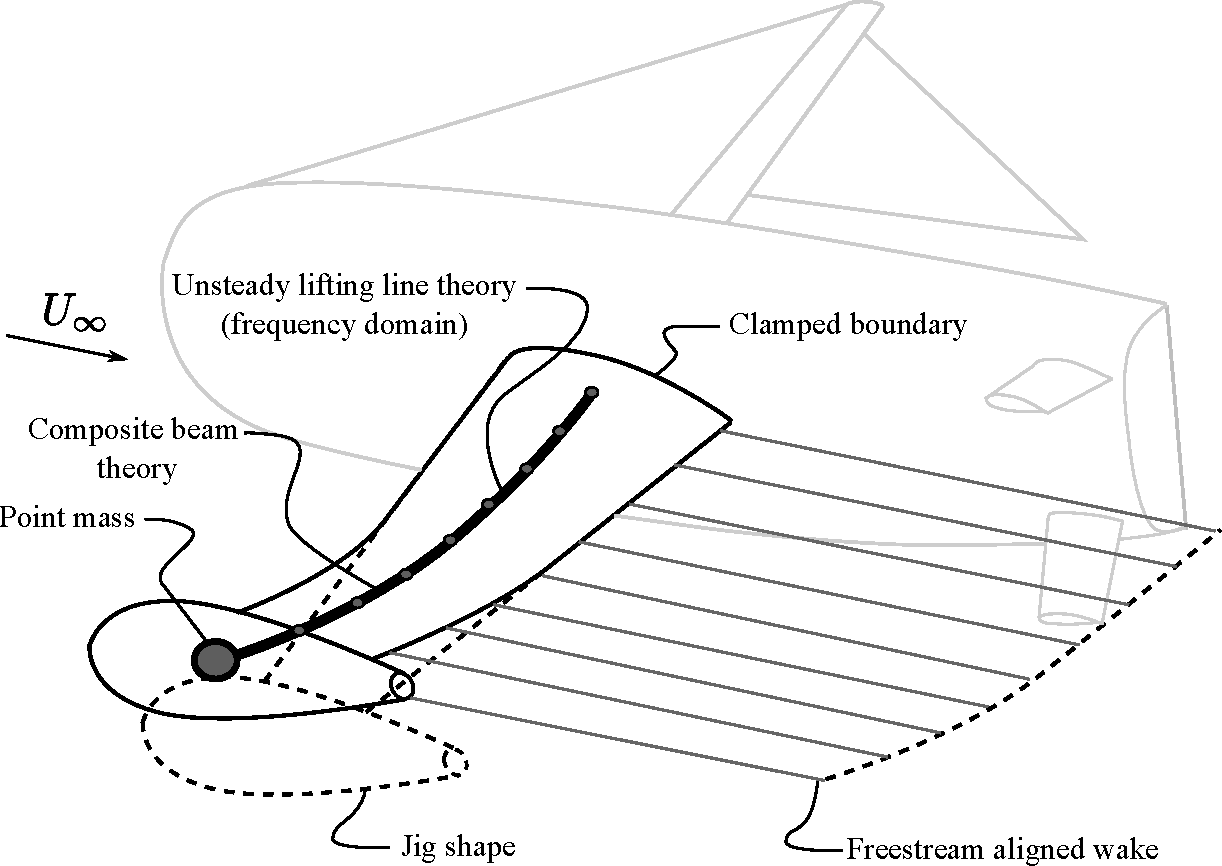
\includegraphics[width=1.0\linewidth,clip,trim={0cm 0cm 0cm 10cm}]{keel-dcfoil.pdf}
    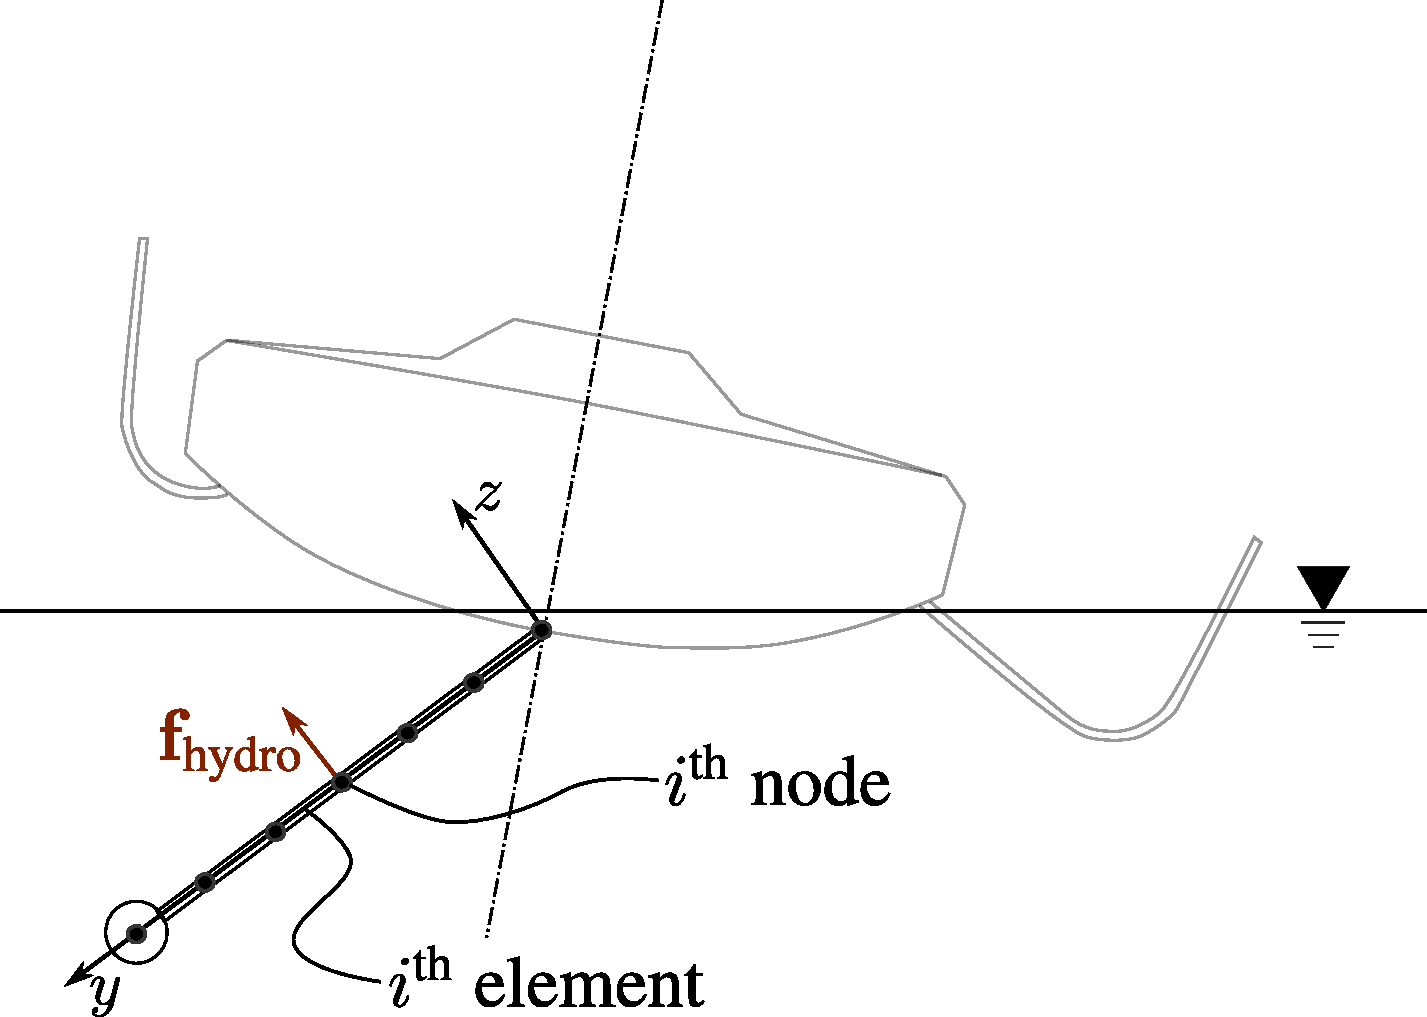
\includegraphics[width=0.5\linewidth,clip,trim={0cm 0cm 0cm 0cm}]{dcfoilkeelfrontview.pdf}
    \caption{\label{fig:keel-dcfoil}
        DCFoil modeling approach for an appendage
    }
\end{figure}

\clearpage
\tableofcontents
\clearpage
% ==============================================================================
%                                 ACRONYMS
% ==============================================================================
\section*{Acronyms}
\begin{acronym}
    \acro{AD}{algorithmic differentiation}
    \acro{CFD}{computational fluid dynamics}
    \acro{CSD}{computational structural dynamics}
    \acro{FSI}{fluid-structure interaction}
    \acro{IMO}{International Maritime Organization}
    \acro{ITTC}{International Towing Tank Conference}
    \acro{EEDI}{Energy Efficiency Design Index}
    \acro{SEEMP}{Ship Energy Efficiency Management Plan}
    \acro{PDE}{partial differential equations}
    \acro{ODE}{ordinary differential equations}
    \acro{DIC}{Digital Image Correlation}
    \acro{RK}{Runge--Kutta}
    \acro{EA}{elastic axis}
    \acro{CP}{center of pressure}
    \acro{CG}{center of gravity}
    \acro{KS}{Kreisselmeier--Steinhauser}
    \acro{DOF}{degrees of freedom}
    \acro{AR}{aspect ratios}
    \acro{BFF}{body-freedom flutter}
    \acro{LLT}{lifting line theory}
    \acro{WMO}{World Meteorological Organization}
    \acro{CFRP}{carbon fiber-reinforced plastic}
    \acro{UD}{uni-directional}
    \acro{PMC}{polymer matrix composite}
    \acro{RPM}{revolutions per minute}
    \acro{TE}{trailing edge}
    \acro{LE}{leading edge}
    \acro{MDO}{multidisciplinary design optimization}
    \acro{FFD}{free-form deformation}
    \acro{RAO}{response amplitude operator}
    \acro{FRF}{frequency response function}
    \acro{FEM}{finite element method}
\end{acronym}
\clearpage
%------------------------------------------------------------------------------
\section{Coordinate system}
% 
The appendage coordinate system is flow is in the $x$-direction, span is in the $y$-direction, and the vertical direction is $z$.

%------------------------------------------------------------------------------
\clearpage
\section{Discretization}
\subsection{Structural model}
% 
The local beam model uses the spanwise direction as $x$ (subscript 1), the chordwise direction as $y$ (subscript 2), and the vertical direction as $z$ (subscript 3).
It is transformed to the global coordinate system by the rotation matrices.
The rotation matrices are
\be
\mbf{T}
=
\ee
\subsubsection{Beam finite element}
% 
The composite beam model uses the well-known slender beam parameters $EI_s$, $GJ_s$, $EA_s$, and additionally $S_s$ and $K_s$ to account for structural warping of non-circular cross sections and material bend-twist coupling, respectively.
No axial coupling to other degrees of freedom (DOF) is currently considered.
The beam is discretized into 2-noded elements with 9 displacement DOFs denoted $u$, $v$, $w$, $\phi$, $\theta$, $\psi$, $\phi'$, $\theta'$, $\psi'$.
% 
\subsubsection{Beam parameters for composite materials via CLT}
% 
The beam parameters are computed from classical lamination theory (CLT) for composite plates using the high aspect ratio plate model from \citet{Weisshaar1985}.
\be
EI = c\left( D_{11} - \frac{D_{12}^2}{D_{22}}\right)      , \quad
GJ = 4c \left(D_{66} - \frac{D_{26}^2}{D_{22}}\right)     , \quad
K  = 2c \left(D_{16} - \frac{D_{26}D_{12}}{D_{22}}\right)
\ee
These relations do not restrict chordwise rigidity (camber), but they do assume zero chordwise moment.
\citet{LOTTATI1985} used the chordwise rigid relations, which simplifies the algebra.

The flexural stiffnesses $D_{ij}$ (6x6 matrix) come via CLT
\begin{align}
    D_{11} & = Q_{11}m^4 + 2\left( Q_{12}+2Q_{66}\right)n^2m^2 + Q_{22}n^4                               \\
    D_{22} & = Q_{11}n^4+2\left( Q_{12} + 2Q_{66}\right)n^2m^2 + Q_{22}m^4                               \\
    D_{66} & = \left(Q_{11} +Q_{22} - 2Q_{12}-2Q_{66}\right)n^2m^2 + Q_{66}\left( n^4 + m^4 \right)      \\
    D_{12} & = \left(Q_{11} +Q_{22} - 4Q_{66}\right)n^2 m^2 + Q_{12}\left( n^4 + m^4 \right)             \\
    D_{16} & = \left(Q_{11} +Q_{22} - 2Q_{66}\right)n m^3 + \left(Q_{12} - Q_{22} + 2Q_{66}\right) n^3 m \\
    D_{26} & = \left(Q_{11} +Q_{22} - 2Q_{66}\right)n^3 m + \left(Q_{12} - Q_{22} + 2Q_{66}\right) n m^3
\end{align}
where
\be
m= \cos\theta_f,
\quad
n= \sin\theta_f.
\ee
%
The reduced in-plane stiffness coefficients $Q_{ij}$ for the individual plies are
%
\be
Q_{11} = \frac{E_1}{1-\nu_{12}\nu_{21}}, \quad
Q_{12} = \frac{\nu_{12} E_2}{1-\nu_{12}\nu_{21}}, \quad
Q_{22} = \frac{E_2}{1-\nu_{12}\nu_{21}}, \quad
Q_{66} = G_{12}
\ee

The following are numerical methods for computing structural properties of airfoils.
The sectional mass properties are
\be
& m_s & = \int_{0}^{c} \rho \left(Z_u - Z_\ell \right)  dx \doteq \tn{kg-m}^{-1}
\\
& I_s & = \int_{0}^{c}\int_{0}^{t_{\tn{max}}} r^2 dm
\ee
where we evaluate the integrals numerically.

The sectional geometric properties are\footnote{The torsional constant is NOT the same as the polar moment}
\be
& \bar{z} & =\frac{1}{A} \int_0^c \frac{1}{2}\left[Z_u^2-Z_{\ell}^2\right] d x \\
& I & =\int_0^c \frac{1}{3}\left[\left(Z_u-\bar{z}\right)^3-\left(Z_{\ell}-\bar{z}\right)^3\right] d x \\
& J &= \int \\
\ee
and torsional warping resistance due to tension from \citet{LOTTATI1985} is
\be
S = \int_{-b}^b D_{22} x_a^2 d x, \quad\tn{where } x_a = x - ba
\ee
\subsubsection{Structural damping}
% 
We use a proportional (Rayleigh) damping model, which is commonly used for multi-DOF structures because of mathematical conveniences
\ben
\mbf{C_s} = \alpha \mbf{M_s} + \beta \mbf{K_s}.
\een
The mass proportional damping decreases with increasing response frequency whereas the stiffness proportional damping increases.
We specify $\zeta = 2\%$ damping ratio at an undamped, in-vacuum, natural frequency giving
% We specify $\zeta = 2\%$ damping ratio at the minimum and maximum undamped, in-vacuum, natural frequencies to determine the unknown constants.
% This simplifies the solution for the mass-proportional and stiffness-proportional constants to
% \ben
% \alpha = \frac{2 \zeta}{\omega_{\tn{min}} + \omega_{\tn{max}}} \qquad \beta = \omega_{\tn{min}} \omega_{\tn{max}} \alpha
% \een
% where $\omega_{\tn{min}}$ and $\omega_{\tn{max}}$ are the undamped natural frequencies in radians per second determined from modal analysis.
% All response frequencies between $\omega_{\tn{min}}$ and $\omega_{\tn{max}}$ are damped by a smaller amount.
$\beta = {2 \zeta}/{\omega_{\tn{max}}}$
where $\omega_{\tn{max}}$ is the highest undamped, in-vacuum, natural frequency in radians per second determined from modal analysis--in this paper, the fourth natural mode.

A few options are available but we typically use the stiffness proportional method ($\alpha=0$) because response frequencies in water tend to be on the lower side;
we want to avoid artificial overdamping of critical hydroelastic modes with $\omega < \omega_{\tn{max}}$.
Structural damping is typically small compared to hydrodynamic damping so its main role is as a margin of stability if fluid damping is close to zero, thus accuracy of the structural damping model is not critical.
% 
\subsection{Hydrodynamic loads}
% 
\subsubsection{Steady lifting line}
% 
The lifting line model derives from~\citet[Ch. XI]{Glauert1983a} and works for arbitrary chord.
Specifically, we are after sectional lift slopes ($\textstyle c_{\ell_\alpha} = \tn{d}c_\ell/\tn{d}\alpha$).
We assume
\begin{itemize}
    \item the chord is small compared to the span,
    \item the wing is symmetric about the centerline,
    \item span is straight and orthogonal to the freestream
    \item trailing vortices are shed from the trailing edge and align with the freestream (no sweep or dihedral)
\end{itemize}

The wing is represented by superimposing ``horseshoe'' systems of vortex lines (analagous to a wire with electrical current).
This is because the circulation across a wing is not constant.
The free vortex system is a sheet of trailing vortices springing from the trailing edge.
The induced velocity of an element of the line ($ds$) at point $P$ from one vortex line of constant strength $\Gamma$ is
\be
dq = \frac{\Gamma}{4 \pi r^2} \sin(\theta) ds
\ee
but in practice, one would solve this as an integral over the entire vortex line, so we will build up to the full wing.

% We know the forces to be
% \begin{align}
%      & L = \int_{-s/2}^{s/2} \rho \Uinf \Gamma(y) dy          \\
%      & D_i = \int_{-s/2}^{s/2} \rho \Uinf w(y)  \Gamma(y) dy
% \end{align}
% where $s$ is total span.
To begin solution, we first assume the circulation is the Fourier series\footnote{\citet{Kerwin2010} use $\tilde{y}$ as $\theta$}
\be
\Gamma(y) = 2 \Uinf s \sum_{n=1}^{\infty} a_n \sin \left( n \theta \right)
\quad \tn{where }
y = -\frac{s}{2}\cos(\theta)
\quad \tn{and }
\theta \in \left[-\frac{\pi}{2},\frac{\pi}{2}\right]
.
\ee
The difficulty is now determining the Fourier coefficients $a_n$ so we need some relations for $\Gamma(y)$ to solve it.

One relation is the equation for the normal induced velocity (downwash velocity) at a point along the span
\be
\label{eq:downwash}
w(y) = \frac{1}{4\pi}
\int_{-s/2}^{s/2} \frac{\dd{\Gamma}{\eta} }{y - \eta} d\eta
=
\boxed{
    -\Uinf \sum_{n=1}^{\infty} \frac{n a_n \sin \left( n \theta \right)}{\sin(\theta)}
}
\ee
where $\eta$ is the spanwise coordinate and $s$ is total span.
We skipped a few steps in the derivation~\cite[Sec.~3.7]{Kerwin2010}.

The second relation is from sectional lift as a function of circulation.
Recall that the circulation at a section (derived from Kutta-Joukowski lift theorem) is
\be
\label{eq:circulation}
\Gamma(y) = \half c_\ell c \Uinf
=\half a_0 c \left(\Uinf \alpha - w(y)\right)
\ee
where we made use of $c_\ell = a_0 \alpha_{\tn{eff}} = a_0 \left(\alpha - w/\Uinf\right)$.
After substitution of the Fourier series form and combining Equations~\eqref{eq:downwash} and~\eqref{eq:circulation}, we end up with
\be
\label{eq:circulation2}
\sum_{n=1}^{\infty} a_n \sin(n\theta) \left(n\mu + \sin(\theta)\right)
=
\mu \alpha \sin(\theta)
\quad \tn{where }\mu(\theta) = \frac{a_0 c(\theta)}{ 4 s}
\ee
where the impact of geometric twist can be captured via $\alpha = \alpha_0 + f(\theta)$ where $f(\theta)$ is the twist as a function of the spatial variable.

Here's the digestion of the Julia code which does the numerical solution of Equation~\eqref{eq:circulation2} but symmetrically about the centerline.
\begin{align*}
     & \tilde{y} = \left[
        0,\frac{\pi}{2}
        \right] \quad \tn{of size nNodes}
    \\
     & \mbf{n} = \left[1:2:2\times\tn{nNodes}\right]
    \\
     & \mbf{c} = c  \sin(\tilde{y}) \quad \tn{(parametrized vector leading to elliptical planform)}
    \\
     & \mbf{b} = \frac{\pi}{4} \frac{\mbf{c}}{s/2} \alpha \sin(\tilde{y}) \quad \tn{(RHS of Equation~\eqref{eq:circulation2} in vector form)}
    \\
     & \tilde{y}n = \tilde{y} \otimes \mbf{n} \quad \tn{(outer product)}
    \\
     & \mbf{A_0} = \begin{bmatrix}
                       |               & |                        \\
                       \sin(\tilde{y}) & \sin(\tilde{y}) & \cdots \\
                       |               & |
                   \end{bmatrix} \quad \tn{(square matrix of $\sin(\tilde{y})$)}
    \\
     & \mbf{A_1} = \frac{\pi}{4} \frac{\mbf{c}}{s/2} \otimes \mbf{n} \quad \tn{(outer product representing $n\mu$ on LHS)}
    \\
     & \mbf{A} = \sin(\tilde{y} n ) \odot \left( \mbf{A_0}+\mbf{A_1} \right)                                                                  \\
     & \mbf{A}\mbf{x} = \mbf{b} \quad \tn{(solve linear system for $\mbf{x} = a_n$)}                                                          \\
     & \Gamma(y) = 4 \Uinf s/2 \left(\underbrace{\sin(\tilde{y}n)\mbf{x} }_{\tn{mat-vec product}} \right)                                     \\
     & c_\ell = \frac{2\Gamma(y)}{\Uinf {c}}                                                                                                  \\
     & c_{\ell_{\alpha}} = \frac{c_\ell}{\alpha}
\end{align*}

\subsubsection{Flap effects}
The effect of a flap comes from thin airfoil theory and is outlined in \citet{Glauert1924,Glauert1927}.
A parameter $\phi = \cos^{-1}\left(\frac{c_f}{2} -1\right)$ is a parametric variable for flap angle accounting for the length of flap chord $c_f$
The lift slope ratio is
\be
\frac{c_{\ell_\delta}}
{c_{\ell_\alpha}}
=
1 - \frac{\phi - \sin(\varphi)}{\pi}
\ee
and the change in moment (positive nose up) is
\be
c_{mac_{\delta}} = -\frac{1}{4}\sin(\phi) \left( 1 - \cos(\phi)\right)
\ee
\begin{figure}[htbp!]
    \centering
    % reference: trim={<left> <lower> <right> <upper>}
    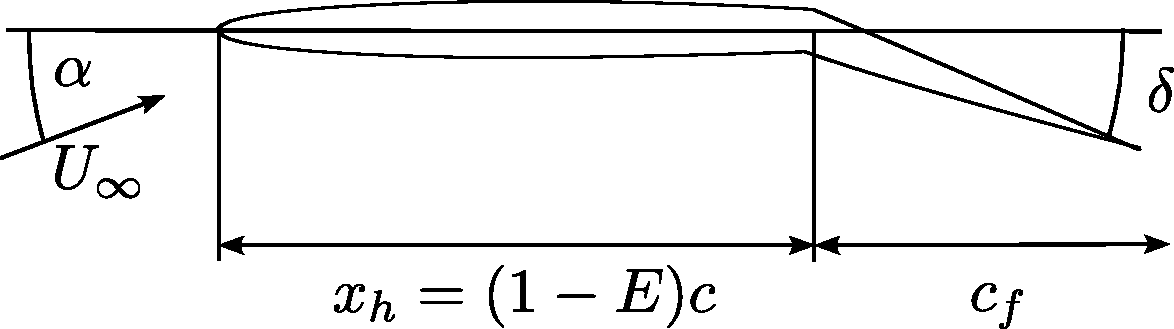
\includegraphics[width=0.5\linewidth,clip,trim={0cm 0cm 0cm 0cm}]{FlapHydrofoil.pdf}
    \caption{\label{fig:Flap}
        Flap diagram
    }
\end{figure}
% NOT DOING THIS, DOUBLE CHECK MATH THOUGH
% Finally, the hinge moment is
% \be
% & H & = k_H (Ec)^2 \rho \Uinf^2
% \\
% & k_H & = \frac{c_{mH_\alpha}}{c_{\ell_\alpha}} c_\ell
% +
% c_{mH_\delta} \delta
% \\
% & c_{mH_{\delta}} & = - \frac{\sin(\varphi) \left(1 - \cos(\varphi) \right)}{4 E^2}
% \left(
% \frac{\pi - \varphi}{\phi}
% -\frac{\sin(\varphi)}{\pi}
% \right)
% \ee

\subsubsection{Extension to unsteady frequency domain}
% 
We are interested in the sectional lift and moments for a harmonically oscillating body.
\citet{Theodorsen:1934} came up with the Theodorsen function $C(k)$ to account for the lag and deficit in forces with a farfield boundary condition.
It is applied as a transfer function to the static hydrodynamics.
\begin{eqnarray}
    \label{eqn:GenFluidTheod}
    \left\{\begin{matrix}
        F_z \\
        M_y
    \end{matrix}\right\}_i =
    -
    \left(
    \left[
        \mbf{m_f}
        \left\{
        \begin{matrix}
            \ddot{w} \\
            \ddot{\psi}
        \end{matrix}
        \right\}
        \right]_i
    +
    \left[
        \mbf{c_f}
        \left\{\begin{matrix}\dot{w} \\ \dot{\psi} \end{matrix}\right\}
        \right]_i
    +
    \left[
        \mbf{k_f}
        \left\{\begin{matrix}w \\ \psi + \alpha_0 \end{matrix}\right\}
        \right]_i
    +
    \left[
        \mbf{\hat{c}_f}
        \left\{\begin{matrix}\dot{w}' \\ \dot{\psi}' \end{matrix}\right\}
        \right]_i
    +
    \left[
        \mbf{\hat{k}_f}
        \left\{\begin{matrix}w' \\ \psi' \end{matrix}\right\}
        \right]_i
    \right)
    \Delta y_i
\end{eqnarray}
where $\Delta y_i$ is the strip width at node $i$, which we assume to be equal to element length.
% 
\begin{equation}
    \label{eqn:FluidMass}
    \mbf{m_f} = \pi \rho_f b^2 \begin{bmatrix}
        1  & ab                                \\
        ab & b^2\left(\frac{1}{8} + a^2\right)
    \end{bmatrix}
\end{equation}
%
\begin{equation}
    \label{eqn:FluidDamp}
    \mbf{c_f}(k) =
    \frac{1}{2}\rho_f b U_0
    \left(
    \begin{aligned}
            \cos(\Lambda)
            \begin{bmatrix}
                \vspace{3mm}c_{\ell_{\alpha}} 2 C(k) & -b \left[2 \pi + c_{\ell_{\alpha}} (1-2a) C (k)\right]     \\
                c_{\ell_{\alpha}} eb 2C(k)           & \frac{b}{2} (1-2a)(2 \pi b - c_{\ell_{\alpha}} 2 eb C (k))
            \end{bmatrix}
            % + \\
            % \sin(\Lambda)\frac{\partial}{\partial y}
            % \begin{bmatrix}
            %     \vspace{3mm}2 \pi b & 2 \pi ab^2                           \\
            %     2\pi ab^2           & 2\pi b^3\left(\frac{1}{8}+a^2\right)
            % \end{bmatrix} % NOTE: this is a repeat of what is in c_f
        \end{aligned}
    \right)
\end{equation}
%
\begin{equation}
    \label{eqn:FluidStiff}
    \mbf{k_f}(k) = \frac{1}{2}\rho_f U_0^2 \cos(\Lambda)
    \left(
    \begin{aligned}
            \cos(\Lambda)
            \begin{bmatrix}
                0 & -C(k)2b c_{\ell_{\alpha}}     \\
                0 & -2eb^2 c_{\ell_{\alpha}} C(k)
            \end{bmatrix}
        \end{aligned}
    \right)
\end{equation}
%
\be
\label{eqn:FluidSweep}
\mbf{\hat{c}_f}(k) =
\frac{1}{2}\rho_f b U_0
\sin(\Lambda)
\left(
\begin{aligned}
        \begin{bmatrix}
            \vspace{3mm}2 \pi b & 2 \pi ab^2                           \\
            2\pi ab^2           & 2\pi b^3\left(\frac{1}{8}+a^2\right)
        \end{bmatrix}
    \end{aligned}
\right)
\ee
%
\begin{eqnarray}
    \mbf{\hat{k}_f}(k) =
    \frac{1}{2}\rho_f b U_0
    \sin(\Lambda)
    \left(
    \begin{aligned}
            U_0 \cos(\Lambda)
            \begin{bmatrix}
                \vspace{3mm} c_{\ell_{\alpha}}2 C (k) & - c_{\ell_{\alpha}} b (1-2a)C(k)          \\
                2ebc_{\ell_{\alpha}} C (k)            & \pi b^2  -c_{\ell_{\alpha}}eb^2(1-2a)C(k)
            \end{bmatrix}
        \end{aligned}
    \right)
\end{eqnarray}
% 
The extra $\hat{\square}$ matrices account for sweep effects on the quasi-steady (damping and stiffness) aerodynamics and are lumped into their respective global matrices if they are in phase with velocity or displacements.

\subsubsection{Free surface effect via desingularized potentials}

The \emph{indirect method} solves for the strengths of the singularities $\sigma$.
The perturbation potential is $\varphi$.
The total velocity potential with steady forward speed ($\Phi = \Uinf x + \varphi $) is some integral of a source distribution $\sigma(\mbf{x}_s)$ over the surface $\Omega$ outside the problem domain
\be
\label{eqn:Indirect}
\boxed{
    \varphi(\mbf{x}) = \iint_\Omega \sigma(\mbf{x}_s) G(\mbf{x}) \tn{d}\Omega
}\\
\varphi(\mbf{x}) = \iint_\Omega \sigma(\mbf{x}_s) \frac{1}{\left| \mbf{x} - \mbf{x}_s \right|} \tn{d}\Omega
.
\ee
We compute the free surface effect using the method of de-singularization first applied in \citet{Cao1991}.
The boundary conditions give rise to the following boundary integral equations (these are also Fredholm integrals of the first kind)
\beq
\label{eqn:BCs}
&
\iint_{\Omega}\sigma(\mbf{x}_s)\frac{1}{\left| \mbf{x}_c - \mbf{x}_s \right| } \tn{d} \Omega & = \varphi_0(\mbf{x}_c) \quad \tn{(Dirichlet) } \Gamma_d
\\
& \iint_{\Omega} \sigma(\mbf{x}_s) \pp{}{n}\left(\frac{1}{\left| \mbf{x}_c - \mbf{x}_s\right|}\right)\tn{d} \Omega & = \chi(\mbf{x}_c) \quad \tn{(Neumann) } \Gamma_n
\eeq
In the indirect method, \citet{Cao1991} says the integrals in Equation~\eqref{eqn:BCs} can be replaced by a summation of singularities without loss of accuracy when desingularization distance is appropriate.
\emph{There is no integration nor mapping.}

The fully nonlinear dynamic and kinematic boundary conditions for the free surface (derived from the unsteady Bernoulli equation) are
\be
\label{eqn:FSBC}
& {\pp{\Phi}{t}}
% \underbrace{
+ \half \left| \nabla \Phi \right|^2
% }_{\approx U\pp{\Phi}{x}}
+ gz_f
&=
-\frac{1}{\rho}\left(p - p_{\tn{atm}}\right)
\quad \tn{(dynamic)}
\\
& \DD{\mbf{x}_f}{t} & = \nabla \Phi \quad \tn{(kinematic)}
\ee
Fully nonlinear free-surface formulations have problems with breaking waves.
As such, linearizing and using a body-exact method where the body boundary condition uses the updated wave elevation is better.
The linearized dynamic boundary condition is
\be
\label{eqn:DFSBC}
{\pp{\varphi}{t}} + \Uinf\pp{\varphi}{x} + g z
=
\underbrace{
    -\frac{1}{\rho}\left(p - \patm\right)}_{=0 \tn{ for } z = \eta}
\\
\eta = -\frac{1}{g}
\left(
\pp{\varphi}{t} + \Uinf \pp{\varphi}{x}
\right)
\ee
which you can use after you solve for the perturbation potential $\varphi$ to determine wave elevation~\cite{Hess1967a}.
The linearized kinematic boundary condition is
\be
\label{eqn:KFSBC}
\pp{\varphi}{z} - \pp{\eta}{t} - \Uinf \pp{\eta}{x} = 0 \\
\pp{\eta}{t} = \pp{\varphi}{z} - \Uinf \pp{\eta}{x}
\ee
Combining them gives the unsteady linearized free surface boundary condition for the perturbation potential
\be
\label{eqn:LSFSBC}
\boxed{\Uinf^2 \ppt{\varphi}{x} + g\pp{\varphi}{z}}
= - \left( \ppt{\varphi}{t}
+ 2 \Uinf \frac{\partial^2 \varphi}{\partial x \partial t}
\right)
\ee
which we then need to use to set up the LHS and RHS on $\Gamma_d$.

The linear system to solve comes from the mixed boundary conditions originally in Equation~\eqref{eqn:BCs}.
The result from this are the unknown source strengths $\sigma_i$.
For the linearized free surface boundary condition, we plug Equation~\eqref{eqn:BCs} in to get
\be
\Uinf^2  \iint_{\Omega}\ppt{   }{x}
\left(
\sigma(\mbf{x}_s) \frac{1}{\left| \mbf{x}_c - \mbf{x}_s\right|}
\right)
\tn{d}\Omega
+ g
\iint_{\Omega} \pp{}{z} \left(
\sigma(\mbf{x}_s) \frac{1}{\left| \mbf{x}_c - \mbf{x}_s  \right| }
\right)
\tn{d}\Omega
= 0
\quad \tn{on } z=0 \tn{ (Free surface Dirichlet BC)}
\ee
Looks pretty nasty, right?
We need to evaluate the above equation in each free surface panel.
But you will also have one more equation for the Neumann BC which will represent the body in the flow, that way it's not just solving a null space problem.

% On a quad panel, the idea is to use shape functions $N_i(\xi, \eta)$ in a reference element at the four nodes
% \ben
% \mbf{x} \approx \sum_{i=1}^{4} N_i(\xi, \eta) \mbf{x}_i
% \qquad
% {\sigma}  \approx \sum_{i=1}^{4} N_i(\xi, \eta) {\sigma}_i
% \een
% so we can actually evaluate stuff like Equation~\eqref{eqn:BCs} per panel.
% Hence, in the numerical solution, we find nodal values.
% Equation~\eqref{eqn:BCs} for an element (panel) might look like
% \be
% \Phi_e =
% \iint_{\Omega_e}
% \frac{\sigma(\mbf{x}_s)}{\left|\mbf{x}_f - \mbf{x}_s \right|}
% \tn{d}x \tn{d}y
% =
% \int_{-1}^1\int_{-1}^{1}   \frac{N_i(\xi , \eta)\sigma_i}{\left|\mbf{x}_f - \mbf{x}_i \right|}
% \det(J)\tn{d}\xi \tn{d}\eta
% \ee
% TODO: I think the above is wrong

% Now, extending this logic to a body of $N_B$ nodes and turning the double integral to a single integral, we have the coupled equations on the boundary points $\mbf{x}_i$
% \be
% &\sum_{j=1}^{N_F} \sigma_j \ln{
%     \left|
%     \mbf{x}_i - \mbf{x}_{sj}
%     \right|
% }
% +
% \sum_{j=1}^{N_B} \sigma_j
% \int_{\Gamma_n} \ln{\left|
%     \mbf{x}_i - \mbf{x}_{sj}
%     \right|} \tn{d}\ell
% &=\phi(\mbf{x}_i)
% \quad
% \mbf{x}_i \in \Gamma_d
% \\
% &\underbrace{
%     -\pi \sigma_i +}_{\tn{Panel's self influence } (\mbf{x}_i=\mbf{x}_{sj})}
% \sum_{j=1}^{N_F} \sigma_j \frac{\left(\mbf{x}_i-\mbf{x}_{sj} \right) \cdot \mbf{N}_i }{
%     \left|
%     \mbf{x}_i - \mbf{x}_{sj}
%     \right|^2
% }
% +
% \sum_{j=1, j \neq i}^{N_B} \sigma_j
% \int_{\Gamma_n}  \frac{ \left( \mbf{x}_i - \mbf{x}_{sj} \right) \cdot \mbf{N}_i}{\left|
%     \mbf{x}_i - \mbf{x}_{sj}
%     \right|^2} \tn{d}\ell
% & =\pp{\phi(\mbf{x}_i)}{N}
% \quad
% \mbf{x}_i \in \Gamma_n
% \ee
% Although, I think in 3D the second equation is not necessarily true?

We can write the above in matrix form as
\be
\label{eqn:AIC}
\begin{bmatrix}
    A_{11} \cdots A_{1N} \\
    \vdots \ddots \vdots \\
    A_{N1} \cdots A_{NN}
\end{bmatrix}
\left\{
\begin{matrix}
    \sigma_1 \\
    \vdots   \\
    \sigma_N
\end{matrix}
\right\}
=
\left\{
\begin{matrix}
    b_1    \\
    \vdots \\
    b_N
\end{matrix}
\right\}
\ee
where $N=N_F + N_B$.
From this, we are saying the Dirichlet and Neumann BCs are stacked vertically on the RHS.

% \twocolumn

% Algorithm~\ref{alg:FSBC} is the overall procedure for computing the influence coefficients for a steady-state free surface.
% % 
% \RestyleAlgo{ruled}
% \begin{algorithm}
%     \LinesNumbered
%     % \SetKwComment{Comment}{/* }{ */}
%     \caption{\label{alg:FSBC}
%         Computation of hydrodynamic loads with a steady free surface boundary condition and constant forward speed
%     }
%     \KwData{Grid points (paneling of geometry) and flow speed}
%     \KwResult{Source strengths $\sigma_i$}
%     Pass in (or generate) mesh and panel with node connectivity of control points $\mbf{x}_c$ and source points $\mbf{x}_s$\;
%     Form $\mbf{A}$ matrix from Equation~\eqref{eqn:AIC}\;
%     Form $\mbf{b}$ of the matrix equation~\eqref{eqn:AIC} (i.e., Dirichlet on free-surface Equation \eqref{eqn:LSFSBC} and Neumann on body)\;
%     Solve $\boldsymbol{\sigma} = \mbf{A}^{-1}\mbf{b}$\;
%     Solve for the velocity potential $\Phi$ in each panel using numerical integration on Equation~\eqref{eqn:Indirect}\;
%     Solve for wave elevations from the dynamic condition using $\Phi(\mbf{x})$ in Equation~\eqref{eqn:KFSBC}\;
%     Solve for hydrodynamic loads on the body using Bernoulli's equation and integration of pressures\;
%     % Update desingularization distance $L_d$ and move $\mbf{x}_s$ to new location\;
%     % March one time step (RK4?)\;
% \end{algorithm}
% 

\subsubsection{2D dipole test problem}
Let us consider on $x$ and $z$ dimensions.
If we do a dipole located at $\mbf{x}_0=(0,-1)$ blowing in the negative $x$ direction, the total potential is
\be
\label{eqn:MovingDipole}
\Phi(x,y) = \Uinf x
+
\underbrace{
    \mu G_{\tn{dipole}}(\mbf{x}; \mbf{x}_0)
    +
    \sum_{j=1}^{N_F} {\sigma_j} G_{\tn{source}}(\mbf{x}; \mbf{x}_{sj})
}_{\varphi}
\ee
where $r=\sqrt{(x-x_0)^2 + (z- z_0)^2}$ is the distance from the singularity to the field point.
The linear system from the BC Equation~\eqref{eqn:LSFSBC} is
\beq
\sum_{j=1}^{N_{\tn{panels}}}
\sigma_j
\left(
\Uinf^2
\ppt{G_{\tn{source}}\left(\mbf{x}; \mbf{x}_{sj}\right)}{x}
+ g\pp{G_{\tn{source}}\left(\mbf{x}; \mbf{x}_{sj}\right)}{z}
\right)
=
-\Uinf^2 \mu
\ppt{G_{\tn{dipole}}\left(\mbf{x}; \mbf{x}_0\right)}{x}
- g \mu
\pp{G_{\tn{doublet}}(\mbf{x}; \mbf{x}_0)}{z}
\quad \tn{for } z = 0
\eeq
where $G\left(\mbf{x}; \mbf{x}_s\right)$ is the Green's function for a source at point $\mbf{x}_s$.
Derivatives are solved in the marine dynamics course pack appendix.
This equation must be solved for the unknown source strengths $\sigma_j$ in each panel.

The wave elevation is
\be
\eta(\mbf{x}) = -\frac{\Uinf}{g}\pp{\varphi}{x}
=
-\frac{\Uinf}{g}
\left(
\sum_{j=1}^{N_{\tn{panels}}}\sigma_j \pp{G_{\tn{source}}\left(\mbf{x}; \mbf{x}_s\right)}{x}
+
\mu
\pp{G_{\tn{dipole}}\left(\mbf{x}; \mbf{x}_0\right)}{x}
\right)
\ee

\subsubsection{2D moving dipole test problem}

The previous formulation appeared to have reflecting waves.
In this formulation, we use the unsteady free-surface boundary condition with time marching.
The dipole moves with speed $U(t) = 1-e^{-4t}$ in the positive $x$ direction and has strength $\mu = 1$.
The potential is
\be
\label{eqn:Potential}
\Phi(x,y) = -U(t)x +
\underbrace{
    \mu G_{\tn{dipole}}(\mbf{x}; \mbf{x}_0) + \sum_{j=1}^{N_F} \sigma_j G_{\tn{source}}(\mbf{x}; \mbf{x}_{sj})
}_{\varphi}
\ee

The initial conditions are
\beq
\varphi(\mbf{x},t=0) = 0 \\
\eta(\mbf{x},t=0) = 0
\eeq

The (linearized) free surface boundary conditions are
\beq
\label{eqn:FSBCTime}
\pp{\eta}{t} & = \pp{\varphi}{z} + U(t) \pp{\eta}{x} \\
\pp{\varphi}{t} & = -g \eta +U(t) \pp{\varphi}{x}
\eeq

The boundary value problem is
\beq
\label{eqn:BVP}
\mu G_{\tn{dipole}}(\mbf{x}; \mbf{x}_0) + \sum_{j=1}^{N_F} \sigma_j G_{\tn{source}}(\mbf{x}; \mbf{x}_{sj})
=\varphi_0
\quad \tn{on } z=0
\eeq

Wave elevation comes from the dynamic boundary condition
\be
\eta(\mbf{x},t) = -\frac{1}{g}\left(\pp{\varphi}{t}+ U(t)\pp{\varphi}{x}\right)
\ee

The Euler-Lagrange time-stepping has two steps.
The first step solves the boundary value problem (Equation~\eqref{eqn:BVP} for Dirichlet BCs) at a fixed time $t$.
The second step marches the free surface boundary conditions in time via Equation~\eqref{eqn:FSBCTime}.

The pseudo-code is
\RestyleAlgo{ruled}
\begin{algorithm}
    \LinesNumbered
    % \SetKwComment{Comment}{/* }{ */}
    \caption{\label{alg:FreeSurfaceMarching}
        Solution of the free surface boundary value problem and time marching
    }
    \KwData{Initial boundary conditions $\phi_0$ and wave elevations $\eta=0$}
    \KwResult{Perturbation potentials $\varphi$ and wave elevations $\eta(t)$}
    % \Comment{=== Populate correlation matrix ===}
    \For{$tt=0:dt:t_f$}{
        Setup linear system for $\sigma_j$ from Equation~\eqref{eqn:BVP}\;
        Solve for $\sigma_j = \mbf{A}^{-1}\mbf{b}$\;
        Compute $\varphi = \mu G_{\tn{dipole}} + \sum_{j=1}^{N_F}\sigma_j G_{\tn{source}}$ \;
        March $\varphi,\eta$ in time one step using Equation~\eqref{eqn:FSBCTime} and RK4 integrator\;
    }
\end{algorithm}

\subsubsection{3D dipole test problem}
% The first test problem is a dipole beneath a flat plane with $\varphi=0$ and strength of $\mu=1$.
% This corresponds to infinite Froude number (impulsive start) for the dipole.
% The dipole is at $\mbf{x}_0 = [0,0,-1]$.
% We find $\pp{\varphi}{n}$ on $z=0$.

% The first step is to convert the potential Equation~\eqref{eqn:Indirect} to a summation with one dipole term
% \be
% \varphi(\mbf{x}_f)
% =
% \underbrace{
% \frac{- \mu}{4\pi}\frac{x}{\left| \mbf{x}_f - \mbf{x}_0\right|^{3/2}}
% }_{\tn{dipole}}+
% \sum_{j=1}^{N_F} \frac{\sigma_j}{\left|
%     \mbf{x}_f - \mbf{x}_{sj}
%     \right|}
% \ee
% where $\mbf{x}_{sj}$ are the source points outside the domain.

% If one plugs in the boundary condition $\varphi=0$ on $z=0$, we get the exact solution
% \be
% \varphi(x,y,z)=
% \frac{-\mu}{4\pi}\frac{x}{\left[x^2 + y^2 + \left( z +1\right)^2\right]^{3/2}}
% +
% \underbrace{\frac{\mu}{4\pi}
%     \frac{x}{\left[x^2 + y^2 + \left(z-1\right)^2 \right]^{3/2}}}_{\tn{unknown sources evaluate to the negative image}}
% \ee
% which gives the exact normal velocity on the plane $z=0$ as
% \be
% \left. \pp{\varphi}{n}\right|_{\tn{exact}} =
% \frac{3}{2\pi}\frac{x}{\left(x^2 + y^2 + 1\right)^{5/2}}
% \ee
% The wave elevation is zero (math checks out).

% Now, in the \emph{numerical solution}, we solve a linear system for the unknown $\sigma_j$, and set up integrals to numerically evaluate $\varphi$ and derived quantities from $\varphi$ like $\pp{\varphi}{n}$.
% First, the linear system is
% \be
% \sum_{j=1}^{N_F} \frac{\sigma_j}{\left|
%     \mbf{x}_i - \mbf{x}_{sj}
%     \right|}
% =\frac{x}{4\pi \left| \mbf{x} - \mbf{x}_0\right|^{3/2}}
% \ee
% The normal velocity is
% \be
% \left.
% \pp{\varphi}{n}\right|_{\tn{numerical}}
% =
% \iint_\Omega \pp{}{n}\left(
% \frac{\sigma(\mbf{x}_s)}{\left| \mbf{x}_f - \mbf{x}_s\right|}
% + \frac{x}{4\pi \left| \mbf{x} - \mbf{x}_0\right|^{3/2}}
% \right)
% \tn{d}\Omega
% \ee
% determined from numerical integration.
% The procedure for numerical integration of this quantity is
% \be
% \left. \pp{\Phi}{n}\right|_{\tn{panel}} = \int_{-1}^{1} \int_{-1}^{1}
% \pp{}{n}\left(
% \frac{N_i\sigma_i}{\mbf{x}_f - \mbf{x}_i}
% + \frac{x}{4\pi \left|\mbf{x}_f - \mbf{x}_0 \right|^{3/2}}
% \right)
% \det(J) \tn{d}\xi \tn{d}\eta
% \ee
% So I think we just need the derivative of the inner expression with $\mbf{x}_f$ as the variable to take the derivative of!
% TODO: Do it and then code it up to compare
% Check \citet{Bandyk2009} thesis Appendix B for how to do normal velocity. 
% There is some handy identity...

If we do a dipole located at $\mbf{x}_0=(0,0,-1)$ moving in steady forward speed, the potential is
\be
\label{eqn:MovingDipole}
\Phi = \Uinf x
\underbrace{
-\frac{\mu}{4\pi}\frac{x}{ \left|\mbf{x}_f - \mbf{x}_0\right|^{3}} + \sum_{j=1}^{N_F} \frac{\sigma_j}{\left| \mbf{x}_f - \mbf{x}_{sj}\right|}
}_{\varphi}
\ee
and the linear system is
\beq
\Uinf^2  \iint_{\Omega}\ppt{   }{x}
\left(
\sigma(\mbf{x}_s) \frac{1}{\left| \mbf{x}_c - \mbf{x}_s\right|} \tn{d}\Omega
-\frac{\mu x }{4\pi \left| \mbf{x} - \mbf{x}_0\right|^{3}}
\right)
+ g
\iint_{\Omega} \pp{}{z}
\left(
\sigma(\mbf{x}_s) \frac{1}{\left| \mbf{x}_c - \mbf{x}_s  \right| \tn{d}\Omega}
-\frac{\mu x}{4\pi \left| \mbf{x} - \mbf{x}_0\right|^{3}}
% + \Uinf x
\right)
=\mbf{0}
\tn{ on } z= 0
\eeq
where the LHS came from plugging $\Phi$ into the linearized free surface boundary condition Equation~\eqref{eqn:LSFSBC}.
Turning this into a summation and rearranging to put unknowns on the LHS and knowns on the RHS, we get
\ben
\sum_{j=1}^{N_F}
\left(
\Uinf^2
\ppt{   }{x}
\left(
    \frac{\sigma_j}{\left| \mbf{x}_c - \mbf{x}_s\right|}
    \right)
+ g
\pp{}{z}
\left(
    \frac{\sigma_j}{\left| \mbf{x}_c - \mbf{x}_s  \right| }
    \right)
\right)
=
\Uinf^2 \ppt{ }{x}
\left(
\frac{\mu x}{4\pi \left| \mbf{x} - \mbf{x}_0\right|^{3}}
\right)
+
g\pp{}{z}
\left(
\frac{\mu x}{4\pi \left| \mbf{x} - \mbf{x}_0\right|^{3}}
\right)
\quad \tn{on } z=0
\een
which when we expand the derivative, gives
\beq
\sum_{j=1}^{N_{\tn{panels}}}
\sigma_j
\left(
\Uinf^2
\ppt{G\left(\mbf{x}; \mbf{x}_s\right)}{x}
+ g\pp{G\left(\mbf{x}; \mbf{x}_s\right)}{z}
\right)
\\=
\Uinf^2 \mu\left(
\frac{15x^3}{4\pi \left(x^2 + y^2 + (z+1)^2\right)^{7/2}}
-\frac{9x}{4\pi \left(x^2 + y^2 + (z+1)^2\right)^{5/2}}
\right)
+ g
\left(
\frac{-\mu 3x(z+1)}{4\pi \left(x^2 + y^2 + (z+1)^2\right)^{5/2}}
\right) \quad \tn{for } z = 0
\eeq
where $G\left(\mbf{x}; \mbf{x}_s\right)$ is the Green's function for a source at point $\mbf{x}_s$.
This equation must be solved for the unknown source strengths $\sigma_j$ in each panel.
For completeness the LHS of the above is
\be
\sum_{j=1}^{N_{\tn{panels}}}
\sigma_j
\left(
\Uinf^2 \left( \frac{3 (x-x_s)^2}{\left((x-x_s)^2 + (y-y_s)^2 + (z-z_s)^2\right)^{5/2}}
    - \frac{1}{\left((x-x_s)^2 + (y-y_s)^2 + (z-z_s)^2\right)^{3/2}}
    \right)
-
g
\frac{z-z_s}{\left((x-x_s)^2 + (y-y_s)^2 + (z-z_s)^2\right)^{3/2}}
\right)
\ee

One the source strengths are known, we can evaluate the velocity potential and the normal velocity on the free surface from Equation~\eqref{eqn:MovingDipole}.
In steady state, the wave elevation is
\beq
\eta(\mbf{x}) = -\frac{1}{g}
\left(
% \pp{\Phi}{t} +
\Uinf \pp{\varphi}{x}
\right)
=
\frac{\Uinf}{g}\left(
-\frac
    {\mu}{4\pi \left(x^2 + y^2 + (z+1)^2\right)^{3/2}}
+
\frac
    {3\mu x^2}
    {4\pi \left(x^2 + y^2 + (z+1)^2\right)^{5/2}}
+ \sum_{j=1}^{N_F}\sigma_j
\frac{x - x_{sj}}{\left( \left(x - x_{sj}\right)^2 + \left(y - y_{sj}\right)^2 + \left(z - z_{sj}\right)^2 \right)^{3/2} }
\right)
\eeq

% In time domain, this is more difficult because time-marching is required.
\onecolumn
%------------------------------------------------------------------------------
\clearpage
\section{Static solution}
The static hydrostructural equation is
\be
\mbf{K}_{ss} \mbf{u}_s   = \mbf{f}_{\tn{hydro}} = \mbf{K}_f \mbf{u}_s
\\
\mbf{r}(\mbf{u}_s) = \left(\mbf{K}_{ss} - \mbf{K}_f\right)\mbf{u}_s  = \mbf{0}
\ee
and we solve it with Newton-Raphson.
The residual Jacobian is
\be
\pp{\mbf{r}(\mbf{u}_s)}{\mbf{u}_s}
=
\mbf{K}_{ss} - \mbf{K}_{f}
\ee

\subsection{Derivative computation}
% 
Now suppose that we want the derivative of several cost functions $\mbf{f}(\mbf{x,u}_s)$, like lift or drag force.
The total derivative as a form of partials \cite[Sec. 6.7.2]{Martins2022} is
\be
\dd{\mbf{f}}{\mbf{x}} =
\pp{\mbf{f}}{\mbf{x}} + \pp{\mbf{f}}{\mbf{u}_s} \dd{\mbf{u}_s}{\mbf{x}}
\\
\label{eqn:Adjoint}
\boxed{
    \underbrace{
        \dd{ \mbf{f}}{\mbf{x}}
    }_{n_f \times n_x}
    = \pp{\mbf{f}}{\mbf{x}}
    -
    \underbrace{\pp{\mbf{f}}{\mbf{u}_s} \left[\pp{\mbf{r}}{\mbf{u}_s}\right]^{-1}
    }_{\boldsymbol{\Psi^\top} (n_f \times n_u)}
    \pp{\mbf{r}}{\mbf{x}}
}
\ee
so to compute the total gradient, we can solve the \emph{adjoint system}
\be
\pp{\mbf{r}}{\mbf{u}_s}^\top \boldsymbol{\Psi}
=
\pp{\mbf{f}}{\mbf{u}_s}^\top
\qquad
\tn{where}
\quad
\boldsymbol{\Psi} = \begin{bmatrix}
    |                   &        & |                       \\
    \boldsymbol{\psi_1} & \cdots & \boldsymbol{\psi_{n_f}} \\
    |                   &        & |                       \\
\end{bmatrix}
\ee
so there are $n_f$ right-hand sides in this equation.
The partial derivative matrices in Equation~\eqref{eqn:Adjoint} are computed through \ac{AD}.
\subsection{Elliptical lift}
It is helpful to compare lift distributions ($L = \int_{-b/2}^{b/2}L'(y) dy$) to the elliptical lift distribution.
An ellipse is
\be
\gamma(y)=\Gamma_0 \sqrt{1-\left(\frac{2 y}{b}\right)^2}
\ee
where the spanwise lift distribution from the Kutta-Joukowski theorem is $L'(y) = \rho \Uinf \gamma(y)$.
Substituting the spanwise circulation into the Kutta-Joukowski theorem and the relation for total lift, we get
\be
L=\int_{-b / 2}^{b / 2} L^{\prime}(y) d y=\int_{-b / 2}^{b / 2} \rho \Uinf \Gamma_0 \sqrt{1-\left(\frac{2 y}{b}\right)^2} d y=\frac{\pi}{4} \rho \Uinf \Gamma_0 b
\ee
where the integral solution comes from integral tables or the geometric observation that the area of an ellipse is $\pi/4$ times the area of the bounding rectangle.

\subsection{Downwash in wake}
The wave elevation in the farfield some distance $x$ is
\be
\zeta(x) = \frac{2\Gamma}{\Uinf}e^{-\nu h} \sin(\nu x)
\tn{ where }
\nu = \frac{g}{\Uinf^2}
\ee
If we use $c_\ell = (\rho \Uinf \gamma) /\left(q c\right)$, the equation becomes
\be
\zeta(x) = c_\ell c e^{\frac{-gh}{\Uinf^2}} \sin\left(\frac{g x}{\Uinf^2}\right)
\ee

The linearized kinematic free-surface condition states
\be
\label{eqn:KFSBC}
\pp{\varphi}{z} =
\Uinf \pp{\zeta}{x}
\ee
and the exponential decay states
\be
\left. \pp{\varphi}{z} \right|_{z=-h} =
\left. \pp{\varphi}{z} \right|_{z=0} e^{-gh/\Uinf^2}
\ee
so the downwash angle due to transverse gravity waves is
\be
\alpha_{i,\tn{wave}} = \frac{ \left. \pp{\varphi}{z} \right|_{z=-h} }{\Uinf}
=
\frac{
-C_{L_M}
}{Fn_c^2} e^{{-2}/{Fn_h^2}}
\cos\left(
\frac{1}{Fn_c^2}\frac{\xi}{c}
\right).
\ee

\subsection{Total drag}

\citet[Fig. 21.3]{carlton2007} and \citet[Fig. 4]{Chernyshev2023} provide references on total drag of ships.
\citet[Fig. 12.2]{Raymer2012} is also a good reference on drag classification.
The ideas from both give us an idea of the calm-water drag of a foiling ship.
In waves, an added resistance component due to radiated waves from the body responding to incident waves must be considered in total drag.
\begin{figure}[htb!]
    \centering
    % reference: trim={<left> <lower> <right> <upper>}
    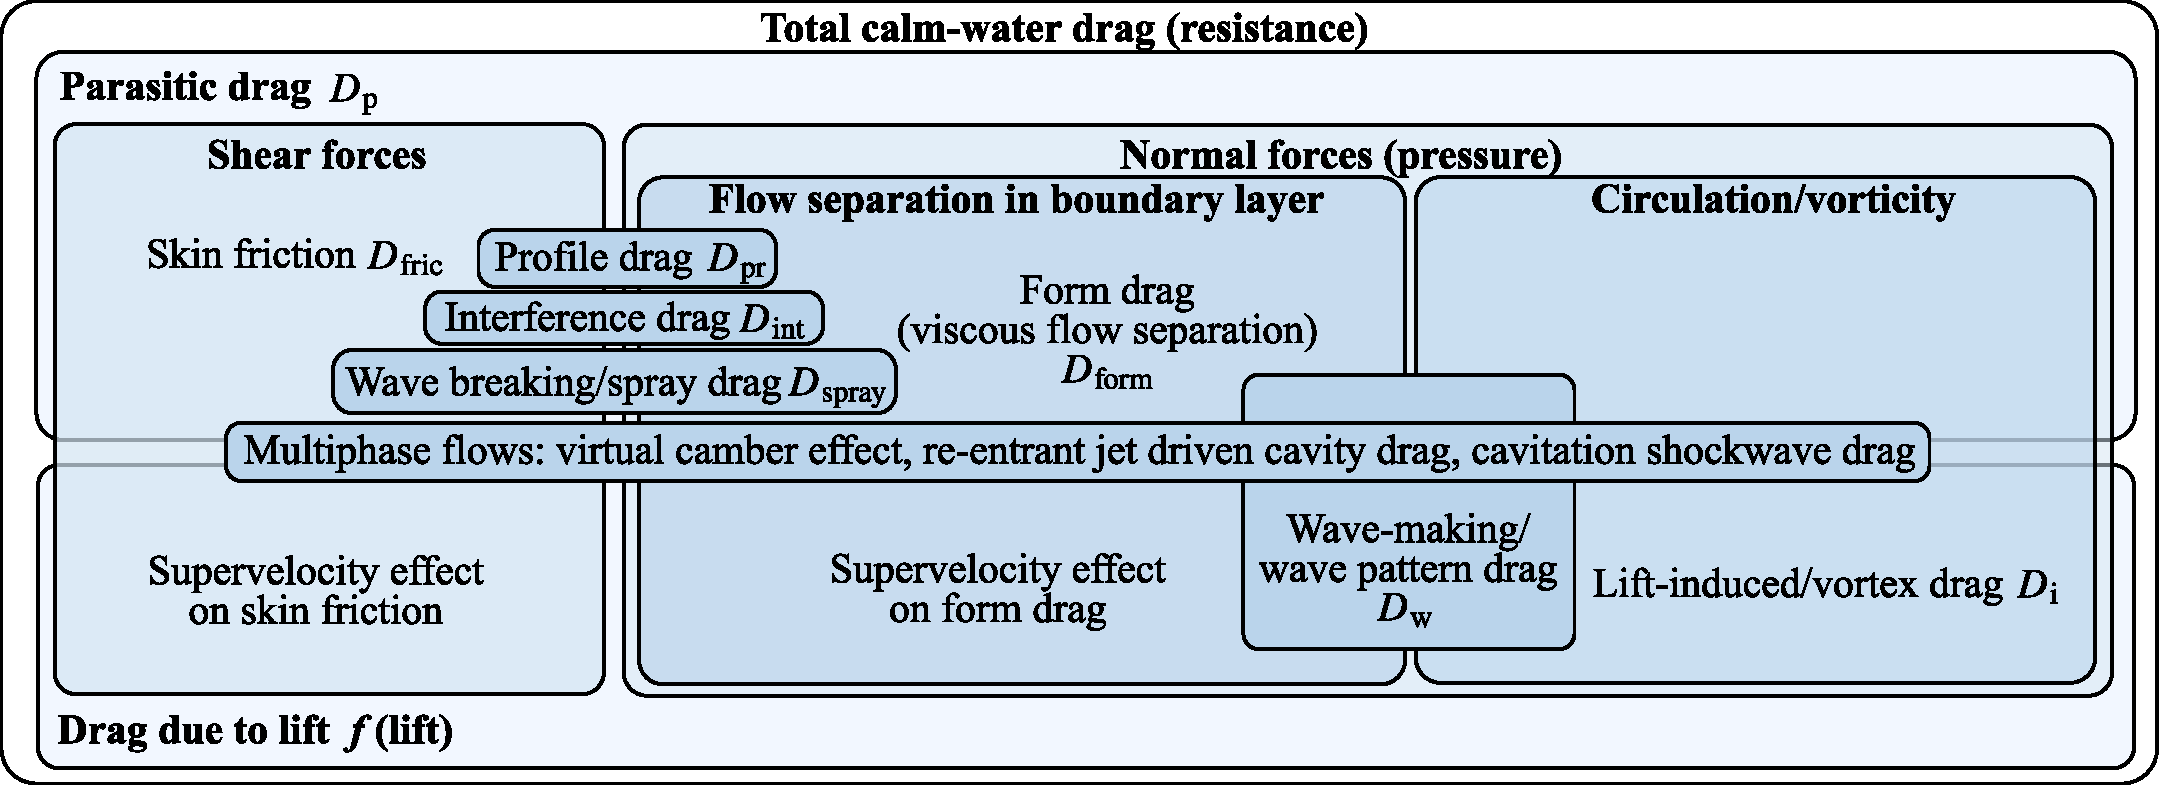
\includegraphics[width=\linewidth,clip,trim={0cm 0cm 0cm 0cm}]{modernDragBuildUp_v2.pdf}
    \caption{\label{fig:HydroDrag}Hydrodynamic drag}
\end{figure}
%------------------------------------------------------------------------------
\clearpage
\section{Forced vibration solution}
\subsection{Governing equations}
The {frequency response solver} separates the magnitudes of static and fluctuating parts of the solution
%
$\mbf{u_{tot}}= \mbf{{u}_{dyn}} + \mbf{u_{stat}}$.
%
% The $\tilde{\square}$ denotes a complex quantity.
The static problem is solved the same way as previously described in, and we solve the dynamic part using the second-order dynamic governing equations for the user-prescribed harmonic forcing vector in the Laplace domain.
We use $j = \sqrt{-1}$.
Equation becomes
\begin{equation}
    \label{eqn:dyn}
    \underbrace{
        \left(-\omega^2  \left(\mbf{M_f + M_s}  \right) +
        j\omega    \left(\mbf{C_f +C_s}\right) + \left(\mbf{K_f + K_s}\right) \right)
    }_{\mbf{D}(\omega)}
    \mbf{\tilde{u}}
    = \mbf{\tilde{f}}.
\end{equation}
%
In this case, we substituted $\mbf{u_{dyn}} =\mbf{\tilde{u}}e^{j \omega  t}$ and $\mbf{f_{ext,dyn}} = \mbf{\tilde{f}}e^{j \omega t}$ into  since we are looking at forced harmonic vibration, and we care more about the steady-state (particular) solution than the initial transience (complementary solution).
The system dynamic matrix ($\mbf{D}(\omega)$), also known as the \emph{impedance matrix}, is not symmetric because of the fluid governing equations.
We solve for the dynamic response with direct inversion of the dynamic matrix.
% The residual for this solver becomes
% \be
% \mbf{r} =
% \underbrace{\mbf{D}(\omega)}_{\mbf{H}(\omega)^{-1}} \mbf{{u}_{dyn}} -
% \mbf{{f}_0}
% \rightarrow \mbf{0}
% \ee
% where $\mbf{H}(\omega)$ is the response amplitude operator matrix that we typically do not solve for since it requires direct inversion.
% The nice property of this is ${\partial r}/{\partial u} = D$.
We solve this equation for a sweep of forcing frequencies ($f = \omega/(2 \pi)$) and then compute the frequency response curves.
The steady-state, frequency response is $\mbf{\tilde{u}} = \mbf{D}^{-1}\mbf{\tilde{f}}$.

The inverse matrix $\mbf{H}(\omega) = \mbf{D}^{-1}(\omega)$ is the RAO or frequency response function (FRF), and it is an nDOF$\times$nDOF matrix computed for every exciting frequency $\omega$.
Knowing the RAO is extremely important for understanding foil response to dynamic loading such as from waves or cavity shedding.

%------------------------------------------------------------------------------
\clearpage
\section{Flutter solution}
\subsection{Governing equations}
% 
The $p$-$k$ method is commonly used in aeroelastic flutter predictions.
The governing equation is solved by assuming a solution of the form
$    \mbf{u} = \tilde{\mbf{u}}e^{pt}$,
%
where $p=\xi + j k$ is our non-dimensional complex eigenvalue, $\xi$ is non-dimensional damping, and $k$ is the reduced frequency.
Eigenvalues are non-dimensionalized using $\Uinf \cos(\Lambda)/\widebar{b}$ where $\widebar{b}$ is the mean semi-chord.
% The complex amplitude ($\tilde{\square}$ terms) is a function of space $\mbf{\tilde{u}}=\mbf{\tilde{u}}(y)$.
The generalized governing discrete equation takes the form
\begin{multline}
    \label{eqn:pkEqn}
    % \underbrace{
    \left[
        \left( \frac{\Uinf\cos(\Lambda)}{\widebar{b}} \right)^2
        p_n^2\left(   \mbf{M_s}   + \mbf{M_f}\right)
        + \frac{\Uinf\cos(\Lambda)}{\widebar{b}}
        p_n\mbf{C_s}
        + \mbf{K_s}
        - \mbf{f_{hydro,quasi}}
        \right]
    % }_{\Delta}
    \mbf{\tilde{u}}_n = \mbf{0}
    \hfill
    \tn{for }n = 1,\ldots,\tn{nmode}.
\end{multline}
where $\mbf{f_{hydro,quasi}}$ are the quasi-steady hydrodynamic forces.
For a non-trivial solution of $\mbf{\tilde{u}}$, the flutter determinant $\det(\Delta)$ is zero, where the bracketed matrix in Equation~\eqref{eqn:pkEqn} is $\Delta$.
We need to find the $p$'s that satisfies the quadratic eigenproblem so that $\det(\Delta) = 0$.
The corresponding $\mbf{\tilde{u}}$ is then the complex eigenvector describing the flutter mode shape.
Simulations sweep flow speed ($\Uinf$).
We can compute in-vacuum natural frequencies by setting all fluid matrices and total damping to zero, giving a linear eigenvalue problem with symmetric matrices;
the eigenvector is the corresponding in-vacuum mode shape.

We can linearize the quadratic eigenvalue problem using the identity $\mbf{I}\dot{\mbf{u}} = \mbf{I}\dot{\mbf{u}}$ to obtain this linear, generalized eigenvalue problem
%
\be
\label{eqn:NgForm}
% A matrix
p_n
\begin{bmatrix}
    \mbf{I} & \mbf{0}                                                         \\
    \mbf{0} & \left( \frac{\Uinf\cos(\Lambda)}{\widebar{b}} \right)^2 \mbf{M}
\end{bmatrix}
\left\{
\begin{matrix}
    \mbf{\tilde{u}} \\
    p_n\mbf{\tilde{u}}
\end{matrix}
\right\}
% B matrix
-
\begin{bmatrix}
    \mbf{0}  & \mbf{I}                                         \\
    -\mbf{K} & - \frac{\Uinf\cos(\Lambda)}{\widebar{b}}\mbf{C}
\end{bmatrix}
\left\{
\begin{matrix}
    \mbf{\tilde{u}} \\
    p_n\mbf{\tilde{u}}
\end{matrix}
\right\}
=
\mbf{0},
\ee
% Note that since fluid-added mass and damping might not be symmetric in marine applications, we
% Equation~\eqref{eqn:NgForm} is the Rodden form~\cite{rodden2011theoretical};
% Other forms are given in~\ref{sec:Eigen}.
We solve Equation~\eqref{eqn:NgForm} following the method of \citet{Zyl2001a} since \citet{Jonsson2020b} has shown the method is suitable and sufficiently robust enough for gradient-based optimization.
The flutter solution method is
\begin{enumerate}
    \item For a given velocity, solve the eigenvalue problem (Equation~\eqref{eqn:NgForm}) for a range of reduced frequencies $k$.
    \item Eigenvalues ($p$) are valid roots if $\Im(p)$ matches the assumed $k$ (matched point solution).
    \item Monitor the difference $\Im(p) - k$. A change in sign indicates a root.
    \item Determine the root by linear interpolation.
\end{enumerate}
where we follow the methodology outlined in~\citet{Jonsson2019a} and \citet[Ch. 3]{Jonsson2020b}.
Since the linear system is quite large, we also use a mode space reduction technique commonly known as the \emph{normal mode} (or modal) method to reduce the size of the matrices and computational cost.

\subsection{Mode tracking}
% 
The mode tracking method prevents mode swapping or hopping during two stages of the flutter analysis:
\begin{enumerate}
    \item during the reduced frequency sweep at a given flight condition and
    \item during the dynamic pressure increments between flight conditions.
\end{enumerate}
We employ the mode tracking method from \citet{Zyl1993}, which uses complex inner products between current and previous eigenvectors to populate a correlation matrix.
$\mbf{\tilde{C}}$.
We search the matrix for largest elements (maximum of one) where the row and column denote previous iteration and current iteration, respectively.
We do this for all modes.
In the frequency sweep, building $\mbf{\tilde{C}}$ is simpler because it is square as the number of eigenvectors between $k$ iterations is the same, resulting in one-to-one mapping.
Between dynamic pressure increments, modes can show up or disappear so $\mbf{\tilde{C}}$ is rectangular.
Therefore, we use a correlation metric (vector $\mbf{c}$) to determine if the computed set of eigenvalues are too far from previously computed values, the process of which is outlined in Algorithm~\ref{alg:ModeTracking}.
Based on the correlation metric value, we either accept or reject the eigenvalues and eigenvectors.
If they are rejected, the dynamic pressure step is halved and we re-run the reduced frequency sweep;
however, the halving process is controlled by a minimum allowed increment $\Delta q_{\tn{min}}$ to prevent excessively long computation times.
If $\Delta q_{\tn{min}}$ is reached, then we accept the roots.

\RestyleAlgo{ruled}
\begin{algorithm}
    \LinesNumbered
    % \SetKwComment{Comment}{/* }{ */}
    \caption{\label{alg:ModeTracking}
        Mode tracking between dynamic pressure increments $q^{(n)}$ and $q^{(n+1)}$ of~\citet{Jonsson2020b} adapted from~\citet{Zyl1993}.
    }
    \KwData{Complex eigenvector matrix $\mbf{V}^{(n)}$ and $\mbf{V}^{(n+1)}$ at succesive $q$'s of size $n_{\tn{dof}} \times n_v^{(n)}$ and $n_{\tn{dof}} \times n_v^{(n+1)}$}
    \KwResult{Vector $\mbf{c}$ of size $n_v^{(n+1)}$ and array $\mbf{m}$ of size $2 \times n_v^{(n+1)}$}
    % \Comment{=== Populate correlation matrix ===}
    Compute ${S_3}_i = {|| \mbf{v}_i^{(n)} ||_2}$ and
    ${S_4}_i = { || \mbf{v}_i^{(n+1)} ||_2}$\;
    % Compute Hadamard product
    % $\mbf{\tilde{C}} = \mbf{V}^{(n)} \circ \mbf{V}^{(n+1)}\quad$\;
    Compute Hadamard product
    $\mbf{C} = | \mbf{V}^{(n)^H} \circ \mbf{V}^{(n+1)}|$\;
    $\mbf{\tilde{C}} = \mbf{C}_{ij}/ \left( {{S_3}_i {S_4}_j }  \right)$\;
    Search $\mbf{\tilde{C}}$ for maximum element\;
    Store row and column indices in array $\mbf{m}$ and then the correlation values in $\mbf{c}$\;
    Set the corresponding rows and columns in $\mbf{\tilde{C}}$ to zero\;
    Repeat process until all elements in $\mbf{\tilde{C}}$ are zero\;
\end{algorithm}


% 
\subsection{Mode space reduction}
%
To reduce the problem size, we use mode space reduction to a reduced set of $N_r$ generalized coordinates.
The displacement field is approximated by
%
\be
\mbf{u} \approx \mbf{Q}_r(y) \mbf{q}(t)
\ee
%
where $\mbf{q} \in \mathbb{R}^{N_r}$ is a vector of retained generalized coordinates and $\mbf{Q}_r \in \mathbb{R}^{N_s \times N_r}$ is a matrix with columns corresponding to eigenvectors.
This is typically called the normal mode method.
One then solves the eigenvalue problem
%
\be
\left( \mbf{K_s} - \omega_i^2 \mbf{M_s}
\right)
\widebar{  \mbf{u} }_i = 0
\ee
%
where $\omega_i$ is the natural frequency.
We compute $\widebar{  \mbf{u} }_i$ and collect them in the matrix
%
\be
\mbf{Q}_r=\left[\begin{array}{cccc}
        \mid                 & \mid                 &        & \mid                     \\
        \overline{\mbf{u}}_1 & \overline{\mbf{u}}_2 & \cdots & \overline{\mbf{u}}_{N_r} \\
        \mid                 & \mid                 &        & \mid
    \end{array}\right]
.
\ee
%
Now the reduced stiffness and mass matrices are
%
\be
\mbf{M_s}_r = \mbf{Q}_r^{\top} \mbf{M_s} \mbf{Q}_r = \mbf{I}_r \in \mathbb{R}^{N_r \times N_r} \\
\mbf{K_s}_r = \mbf{Q}_r^{\top} \mbf{K_s} \mbf{Q}_r = \tn{diag}\left[ \omega_i^2   \right]
\ee
%
and the governing equation reduces to
%
\be
\mbf{M_s}_r \ddot{\mbf{q}} + \mbf{C_s}_r \ddot{\mbf{q}} + \mbf{K_s}_r \mbf{q} - \mbf{Q}_r^{\top} \mbf{f}_{\tn{hydro}} = \mbf{0}
\ee
%

To apply this to the hydrodynamic loads, we obtain from Equation~\eqref{eqn:GenFluid}
%
\be
\mbf{f}_{\tn{hydro},r} =
-\left( \mbf{M_f}_r \ddot{\mbf{u}} + \mbf{C_f}_r \dot{\mbf{u}} + \mbf{K_f}_r \mbf{u}\right)
\ee
%
where the matrices are
%
\be
\mbf{M_f}_r = \mbf{Q}_r^{\top} \mbf{M_f} \mbf{Q}_r \\
\mbf{C_f}_r = \mbf{Q}_r^{\top} \mbf{C_f} \mbf{Q}_r \\
\mbf{K_f}_r = \mbf{Q}_r^{\top} \mbf{K_f} \mbf{Q}_r.
\ee
Note, since cavitating flow leads to non-symmetric matrices, we cannot do all the simplifications \citet{Jonsson2017a} uses.
TODO: OK, this is not actually true because we wouldn't be able to solve in the frequency domain...

% \twocolumn
\subsection{Cost functions}
% 
Reverse mode algorithmic differentiation is applied on the upper-most flutter routine called \texttt{cost\_funcs\_with\_derivs}

\subsubsection{Flutter}
% 
The single flutter constraint uses the damping values ($g = \Re\{p\}$).
We use a two-level KS function aggregation to compute the single constraint first used by \citet{Jonsson2017a}.
It is
%
\be
\label{eqn:KS}
\tn{KS}_{\tn{flutter}} = \tn{KS}\left(\tn{KS} \left( \Re\{p_{n,q}\} \right)\right)
\ee
%
where the first level is over all dynamic pressures $q = 1,\dots,N_q$ and then over all modes $n = 1,\dots,\tn{nmodes}$.
The KS function is
\be
\tn{KS}(\mbf{a}) = a_{\tn{max}} + \frac{1}{\rho}  \ln \sum_i e^{\rho \left( a_i - a_{\tn{max}}\right)}
\ee
where we set the aggregation parameter $\rho=80$ by default.


\subsubsection{Coalescence}

% ==============================================================================
%                         Rigid body dynamics
% ==============================================================================
\section{Rigid body dynamics}
% 
The two coordinate systems are the \emph{earth-fixed} and \emph{body-fixed} (stability) axes, abbreviated EFS and BFS.
DCFoil assumes an equilibrium state is provided (such as from a VPP).
% 
\subsection{Governing equations}
% 
The BFS and EFS origin is at the center of mass of the craft.
Forward is $x$, port is $y$, and up is $z$.
These are different axes from the foil.
There are six degrees of freedom in the BFS denoted $\boldsymbol{\eta} = [\eta_1,\eta_2,\eta_3,\eta_4,\eta_5,\eta_6]^{\top}$.
The six velocities in BFS are $[v_x,v_y,v_z,\omega_x,\omega_y,\omega_z]^{\top}$ where the first three are $\mbf{v}_B$ and the last three are $\boldsymbol{\omega}_B$.
The orientation in EFS are \emph{Euler angles} $[\phi, \theta, \psi]$.
See \Cref{fig:Coordinates}.
\begin{figure}[htb!]
    \centering
    % reference: trim={<left> <lower> <right> <upper>}
    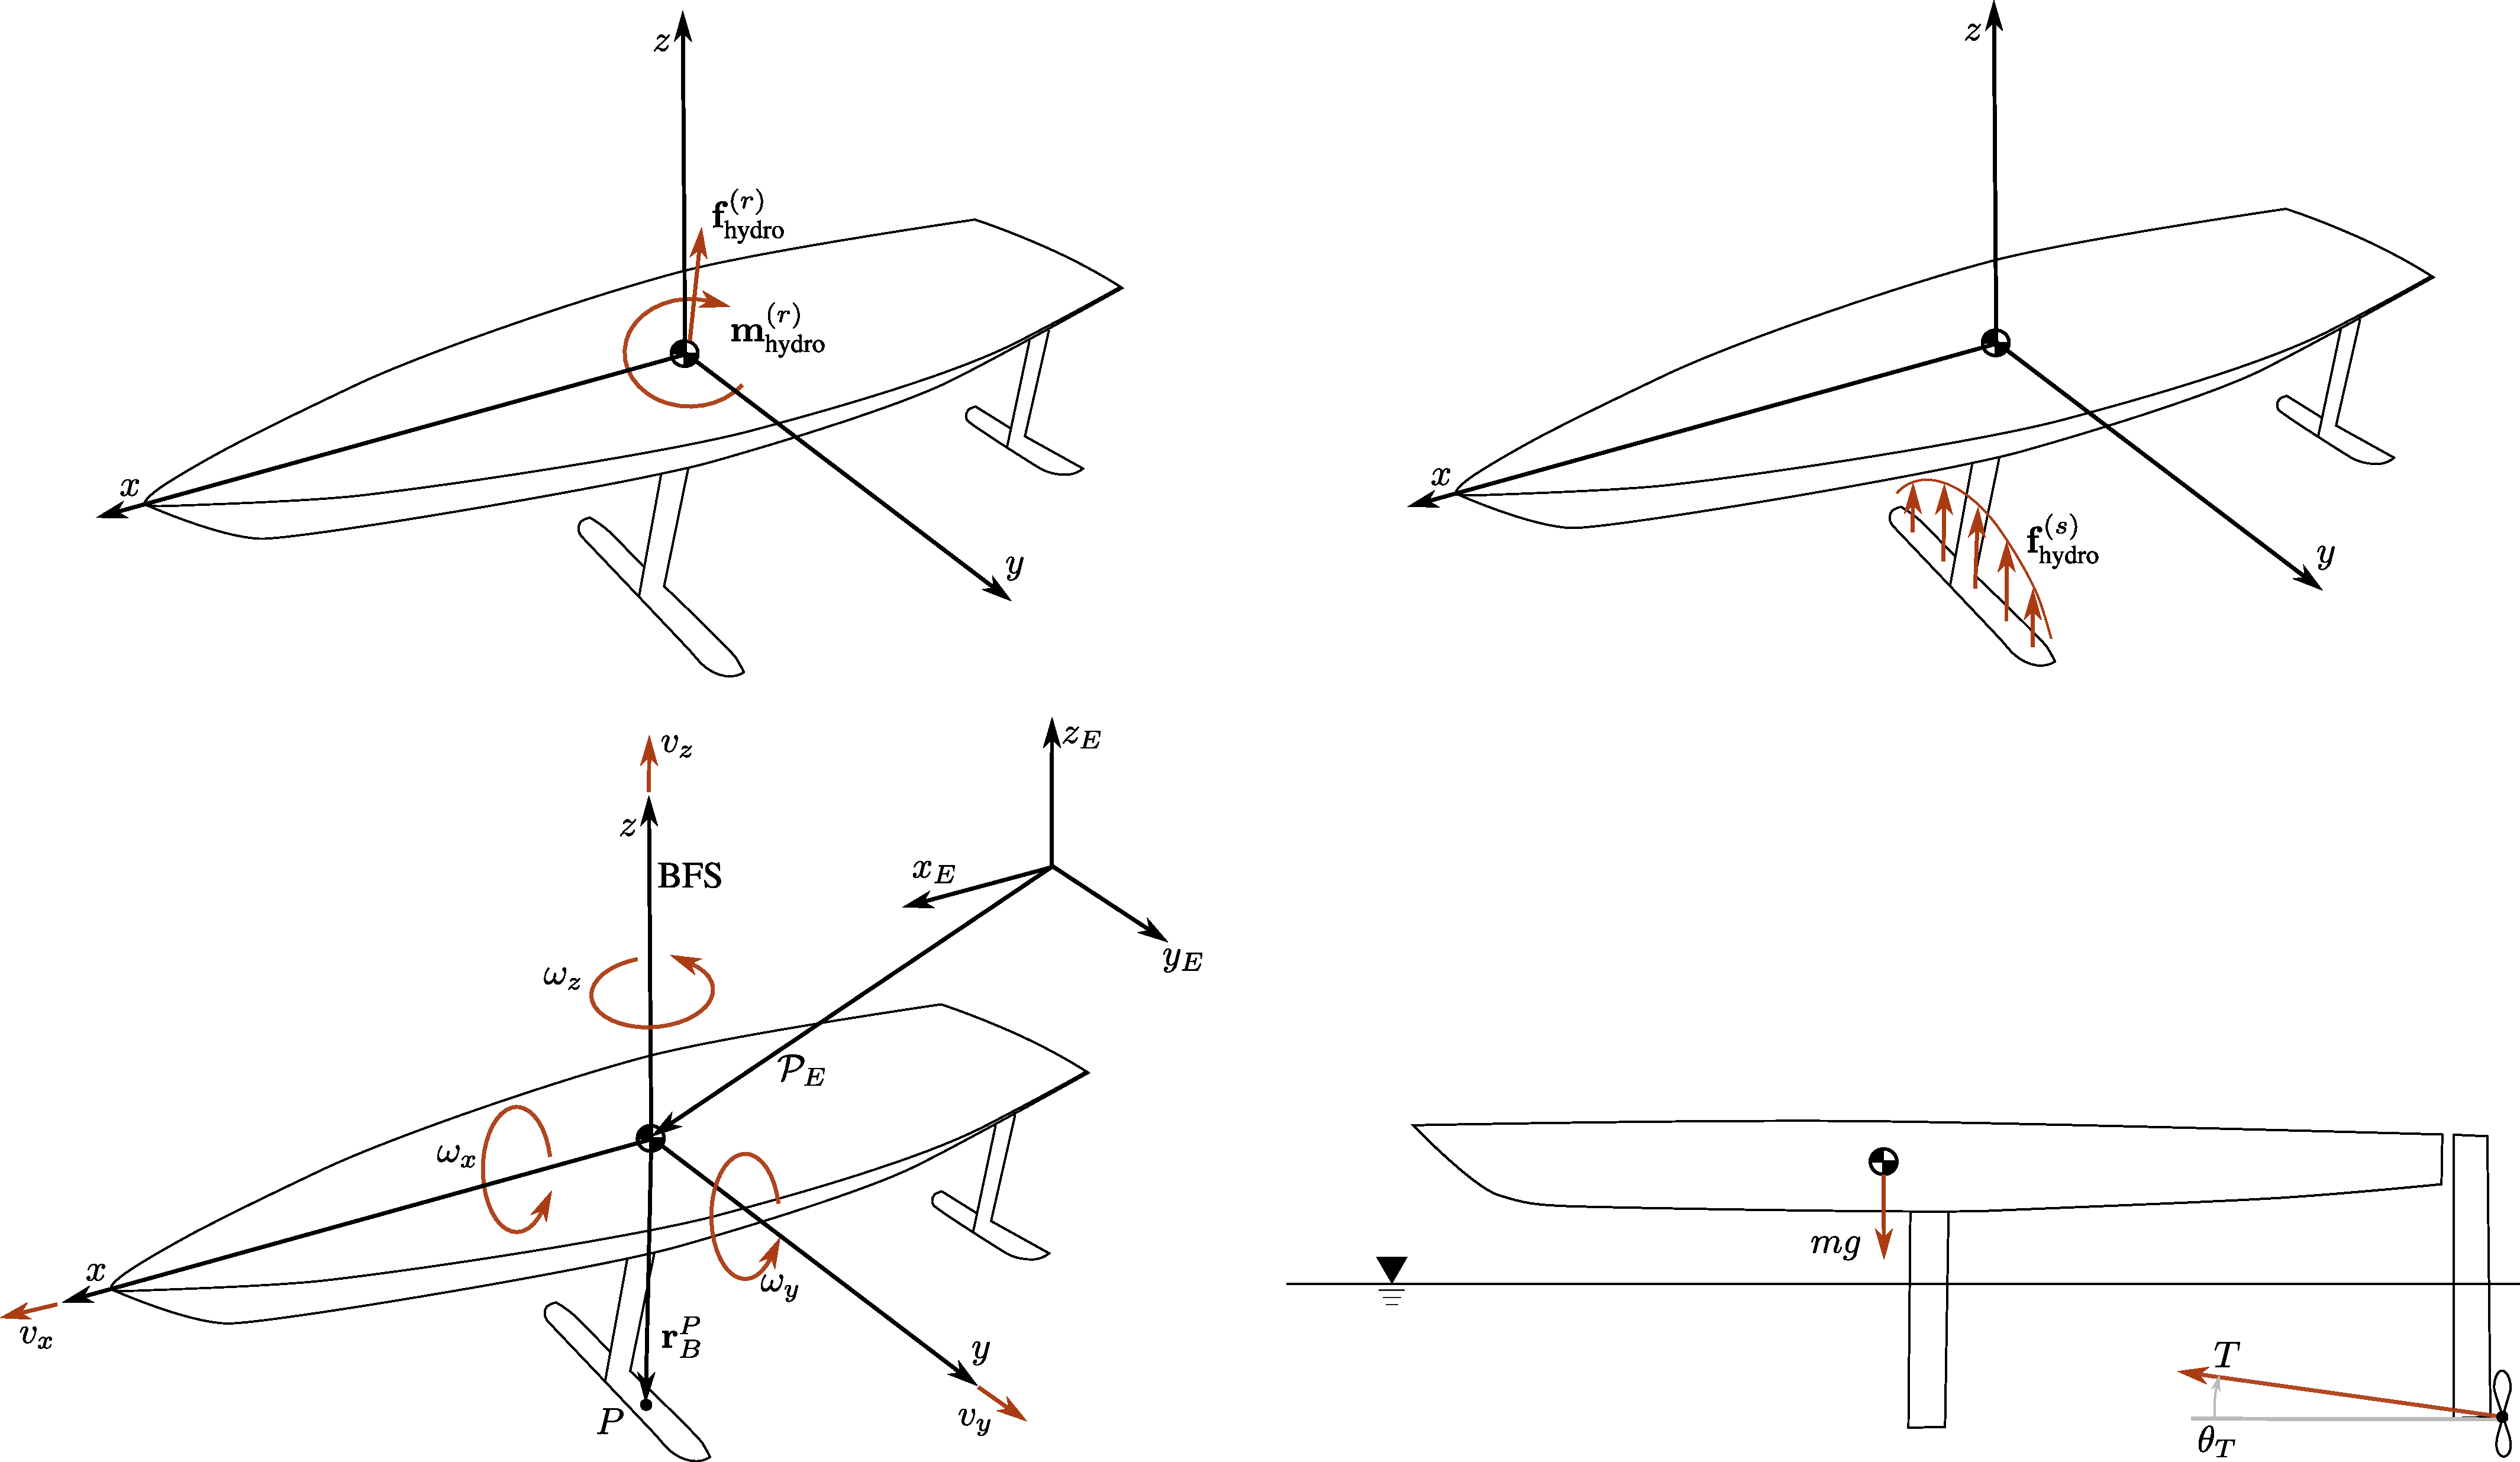
\includegraphics[width=0.6\linewidth,clip,trim={0cm 0cm 37cm 20cm}]{SeakeepingDiagram.pdf}
    \caption{\label{fig:Coordinates}Coordinate system and degrees of freedom}
\end{figure}
\subsection{Kinematics}

A quantity of interest is the vessel velocity in the EFS denoted $\mbf{v}_E$.
Using Euler angles (from EFS obviously), the relationship between BFS and EFS center of mass velocity is
\ben
\mbf{v}_E = \mbf{R}_{BE} \mbf{v}_B.
\een
% 
Now for some point $P$ on the vessel not at the center of mass, the velocity is
\ben
\mbf{v}_E^P = \dot{\mcal{P}}_E + \dot{\mbf{r}}_E^P = \mbf{v}_E + \underbrace{\dot{\mbf{r}}_E^P}_{
    \dot{\mbf{R}}_{BE} \mbf{r}_B^P
},
\een
% 
where ship velocity is $\mbf{v}_E = \dot{\mcal{P}}_E$.
The orientation of the ship in EFS is
\be
\boxed{
    \left\{\begin{array}{c}
        \dot{\phi}   \\
        \dot{\theta} \\
        \dot{\psi}
    \end{array}\right\}=\mbf{T}^{-1} \boldsymbol{\omega}_B=\left[\begin{array}{ccc}
            1 & \sin \phi \tan \theta & \cos \phi \tan \theta \\
            0 & \cos \phi             & -\sin \phi            \\
            0 & \sin \phi \sec \theta & \cos \phi \sec \theta
        \end{array}\right]\left\{\begin{array}{l}
        \omega_x \\
        \omega_y \\
        \omega_z
    \end{array}\right\}}.
\ee
This is the equation you would plug into the time integration scheme.
The \emph{tangential operator} $\mbf{T}(\phi,\theta,\psi)$ based on Euler angles is
\ben
\mbf{T}(\phi, \theta, \psi)=\left[\begin{array}{ccc}
        1 & 0          & -\sin \theta          \\
        0 & \cos \phi  & \sin \phi \cos \theta \\
        0 & -\sin \phi & \cos \phi \cos \theta
    \end{array}\right].
\een
% 
We wrote it this way to not use Euler angles.
Finally, the \emph{transport theorem} is
\ben
\mbf{R}_{B E} \dot{\mbf{v}}_E=\dot{\mbf{v}}_B+\tilde{\boldsymbol{\omega}}_B \mbf{v}_B
\een
% 
where
% 
\ben
\mbf{R}_{B E} \dot{\mbf{R}}_{E B} = \tilde{\boldsymbol{\omega}}_B=\left[\begin{array}{ccc}
        0         & -\omega_z & \omega_y  \\
        \omega_z  & 0         & -\omega_x \\
        -\omega_y & \omega_x  & 0
    \end{array}\right].
\een
\subsection{Inertia}
Total linear momentum is
\ben
\mbf{p}_B=\int_{\mathcal{V}} \mbf{v}_B^P \mathrm{~d} m
= m \mbf{v}_B
\een
and the total angular momentum about the center of mass is
\ben
\mbf{h}_B=\int_{\mathcal{V}} \tilde{\mbf{r}}_B^P \mbf{v}_B^P \mathrm{~d} m
= \mbf{I}_B \boldsymbol{\omega}_B
\een
%
where
\ben
\mbf{I}_B=-\int_{\mathcal{V}} \tilde{\mbf{r}}_B^P \tilde{\mbf{r}}_B^P \mathrm{~d} m=\left[\begin{array}{ccc}
        I_{x x}  & -I_{x y} & -I_{x z} \\
        -I_{y x} & I_{y y}  & -I_{y z} \\
        -I_{z x} & -I_{z y} & I_{z z}
    \end{array}\right]
\een
and $I_{xy} = I_{zy} = 0$ for P/S symmetry.
Example quantities are $\textstyle I_{xx} = \int_{\mcal{V}}\left(y^2+z^2\right) dm$ and $\textstyle I_{yz}=I_{zy}=\int_{\mcal{V}} yz dm$
In EFS, angular momentum is
\ben
\mbf{h}_E=\mbf{R}_{E B} \mbf{h}_B= \underbrace{\mbf{R}_{E B} \mbf{I}_B \mbf{R}_{B E}}_{\mbf{I}_E} \boldsymbol{\omega}_E
\een
\subsection{Equations of motion}
% 
If we plug into Lagrange's equations, we get the equations of motion in BFS
%
\begin{align}
    m\dot{\mbf{v}}_B + m \tilde{\boldsymbol{\omega}}_B\mbf{v}_B                                         & =  \mbf{f}_{\tn{h}B} + \mbf{f}_{pB}  + \mbf{f}_{\tn{g}B} \\
    \mbf{I}_B \dot{\boldsymbol{\omega}}_B+\tilde{\boldsymbol{\omega}}_B \mbf{I}_B \boldsymbol{\omega}_B & = \mbf{m}_{a B}+\mbf{m}_{p B}
\end{align}
where the RHS are hydrodynamic, propulsive, and gravitational loads acting on the center of mass.
% \be
% \begin{bmatrix}
%     m & 0 & 0 & 0   & 0   & 0   \\
%     0 & m & 0 & 0   & 0   & 0   \\
%     0 & 0 & m & 0   & 0   & 0   \\
%     0 & 0 & 0 & I_1 & 0   & 0   \\
%     0 & 0 & 0 & 0   & I_2 & 0   \\
%     0 & 0 & 0 & 0   & 0   & I_3
% \end{bmatrix}
% \ddot{\mbf{\eta}}
% = \sum_i \mbf{f}_i.
% \ee
% 
\subsubsection{Gravitational loads}
% 
The gravitational loads have explicit dependence on vehicle orientation.
\ben
\mbf{f}_{g B}= mg \mbf{R}_{BE} \mbf{e}_3 = \left\{\begin{array}{c}
    -m g \sin \theta          \\
    m g \cos \theta \sin \phi \\
    m g \cos \theta \cos \phi
\end{array}\right\}
\een
\begin{figure}[htb!]
    \centering
    % reference: trim={<left> <lower> <right> <upper>}
    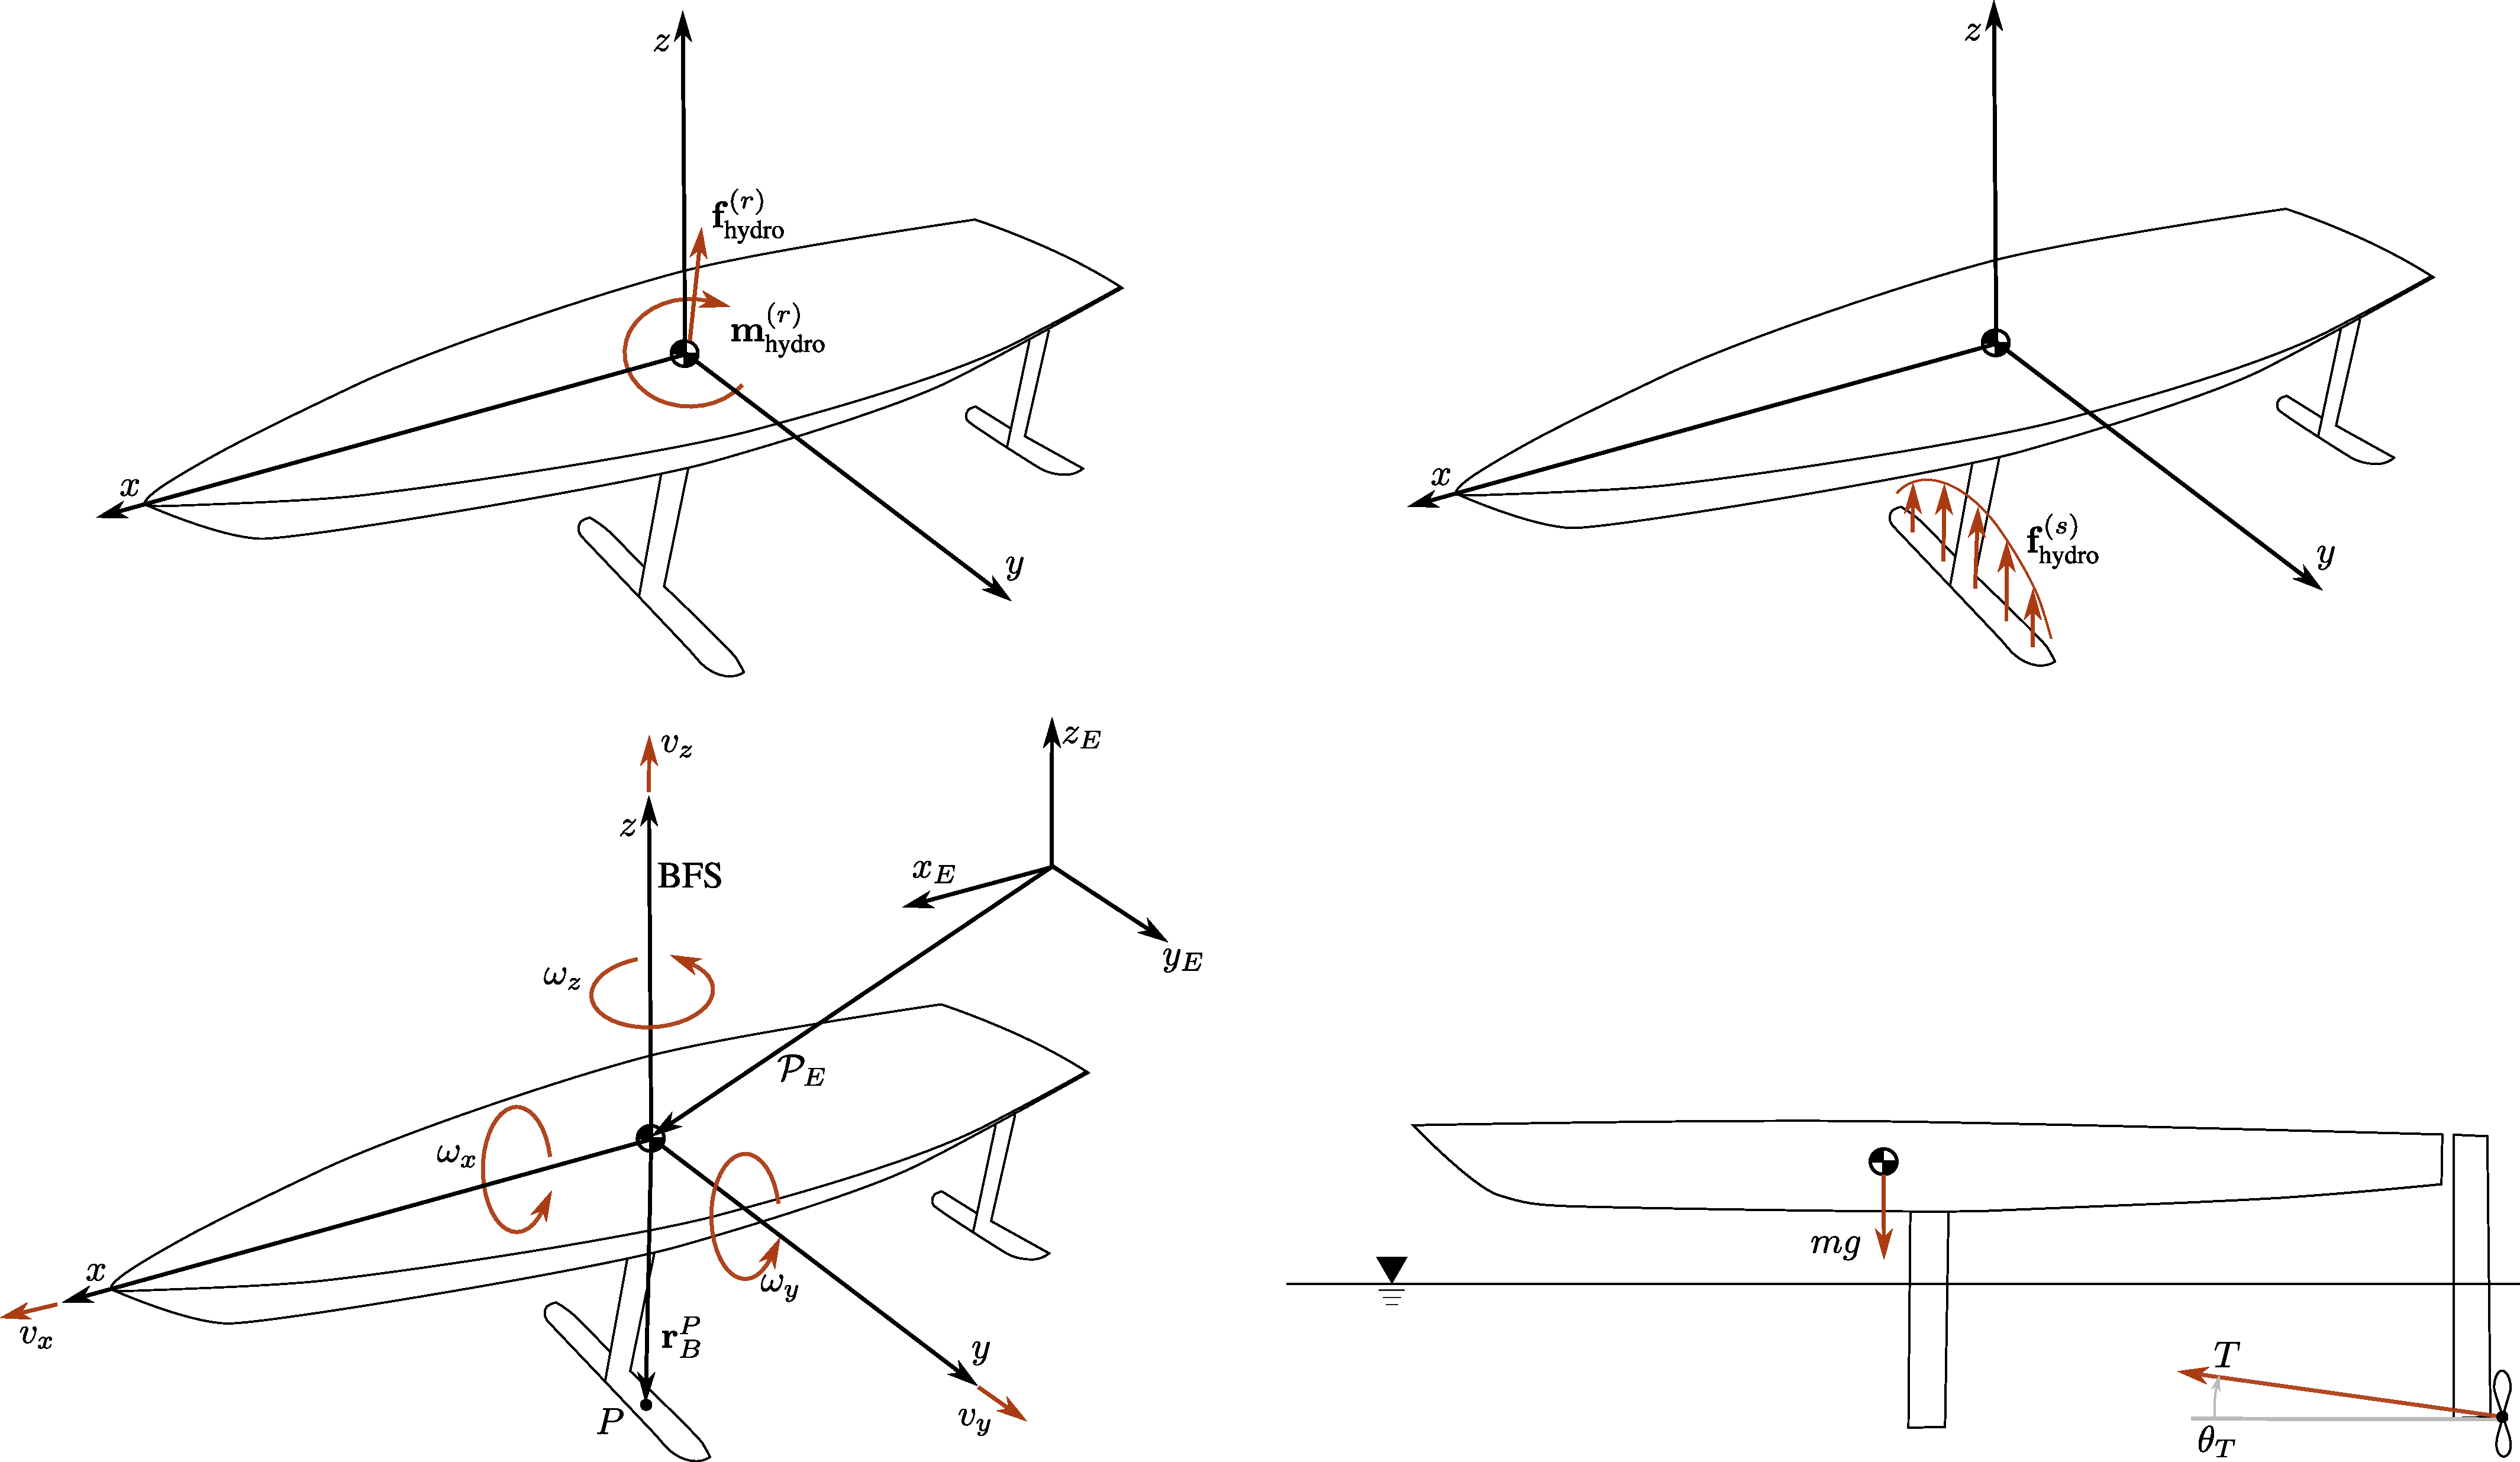
\includegraphics[width=0.6\linewidth,clip,trim={37cm 0cm 0cm 30cm}]{SeakeepingDiagram.pdf}
    \caption{\label{fig:Loads}
        Gravitational and propulsive loads.
    }
\end{figure}

\subsubsection{Propulsive forces}
% 
Assume the propulsion system acts at a point at $(x_T,0,z_T)$ from the CM with some rake angle $\theta_T$.
The propulsive loads are then
\ben
\mbf{f}_{p B}=\left\{\begin{array}{c}
    T \cos \theta_T \\
    0               \\
    -T \sin \theta_T
\end{array}\right\},
\quad
\mbf{m}_{p B}=\left\{\begin{array}{c}
    0                                                 \\
    T\left(z_T \cos \theta_T+x_T \sin \theta_T\right) \\
    0
\end{array}\right\}
\een
% 
\subsubsection{Hydrodynamic loads}
% 
The craft instantaneous angle of attack is
\ben
\alpha(t)=\tan^{-1} \frac{v_z(t)-v_{g z}(t)}{v_x(t)-v_{g x}(t)} \quad \text { and } \quad-{\pi} \leq \alpha \leq {\pi}
\een
where $\mbf{w} = -[v_{gx}, v_{gy}, v_{gz}, \omega_{gx}, \omega_{gy}, \omega_{gz}]^{\top}$ is the disturbance vector of gusts (assume constant).
Leeway angle is
\ben
\beta = \tan ^{-1} \frac{v_y-v_{g y}}{\sqrt{\left(v_x-v_{g x}\right)^2+\left(v_z-v_{g z}\right)^2}} \quad \text { and } \quad-\frac{\pi}{2} \leq \beta \leq \frac{\pi}{2}.
\een
% 
Finally, the velocity vector is
\ben
\mbf{v}_B-\mbf{v}_{g B}=\left\{\begin{array}{c}
    v_x-v_{g x} \\
    v_y-v_{g y} \\
    v_z-v_{g z}
\end{array}\right\}=V_{\mathrm{TAS}}\left\{\begin{array}{c}
    \cos \alpha \cos \beta \\
    -\sin \beta            \\
    \sin \alpha \cos \beta
\end{array}\right\}
\een
where $V_{TAS} = ||\mbf{v}_B-\mbf{v}_{g B} ||$ is the magnitude of the true foiling speed.
The hydrodynamics loads in body axes are
\ben
& \mbf{f}_{h B} & =\frac{1}{2} \rho V_{\mathrm{TAS}}^2 S \mathbf{c}_{\mathbf{f}_B}\left(\mathbf{v}_B-\mathbf{v}_{g B}, \boldsymbol{\omega}_B-\boldsymbol{\omega}_{g B}, \boldsymbol{\delta}_c ; \sigma, \mathrm{Re}\right),                                     \\
& \mbf{m}_{h B} & =\frac{1}{2} \rho V_{\mathrm{TAS}}^2 S \boldsymbol{\Lambda}_{\mathrm{ref}} \mathbf{c}_{\mathbf{m}_B}\left(\mathbf{v}_B-\mathbf{v}_{g B}, \boldsymbol{\omega}_B-\boldsymbol{\omega}_{g B}, \boldsymbol{\delta}_c ; \sigma, \mathrm{Re}\right),
\een
where $\mbf{c}_{\mbf{f}_B}$ and $\mbf{c}_{\mbf{m}_B}$ are the force and moment coefficients, respectively.
The vector $\boldsymbol{\delta}_c$ is the vector of angles of the control surfaces.

The hydrodynamic stability derivatives allow us to tune $\boldsymbol{\delta}_c$ to find incremental changes in the hydrodynamic loads.
\be
& \Delta \mbf{f}_{h B} & = q S \left( \Delta \mbf{c}_{\mbf{f}_B} + \right)
\\
& \Delta \mbf{m}_{h B} & = q S \left( \Delta \mbf{c}_{\mbf{m}_B} + \right)
\ee
% 
\begin{figure*}[htb!]
    \centering
    % reference: trim={<left> <lower> <right> <upper>}
    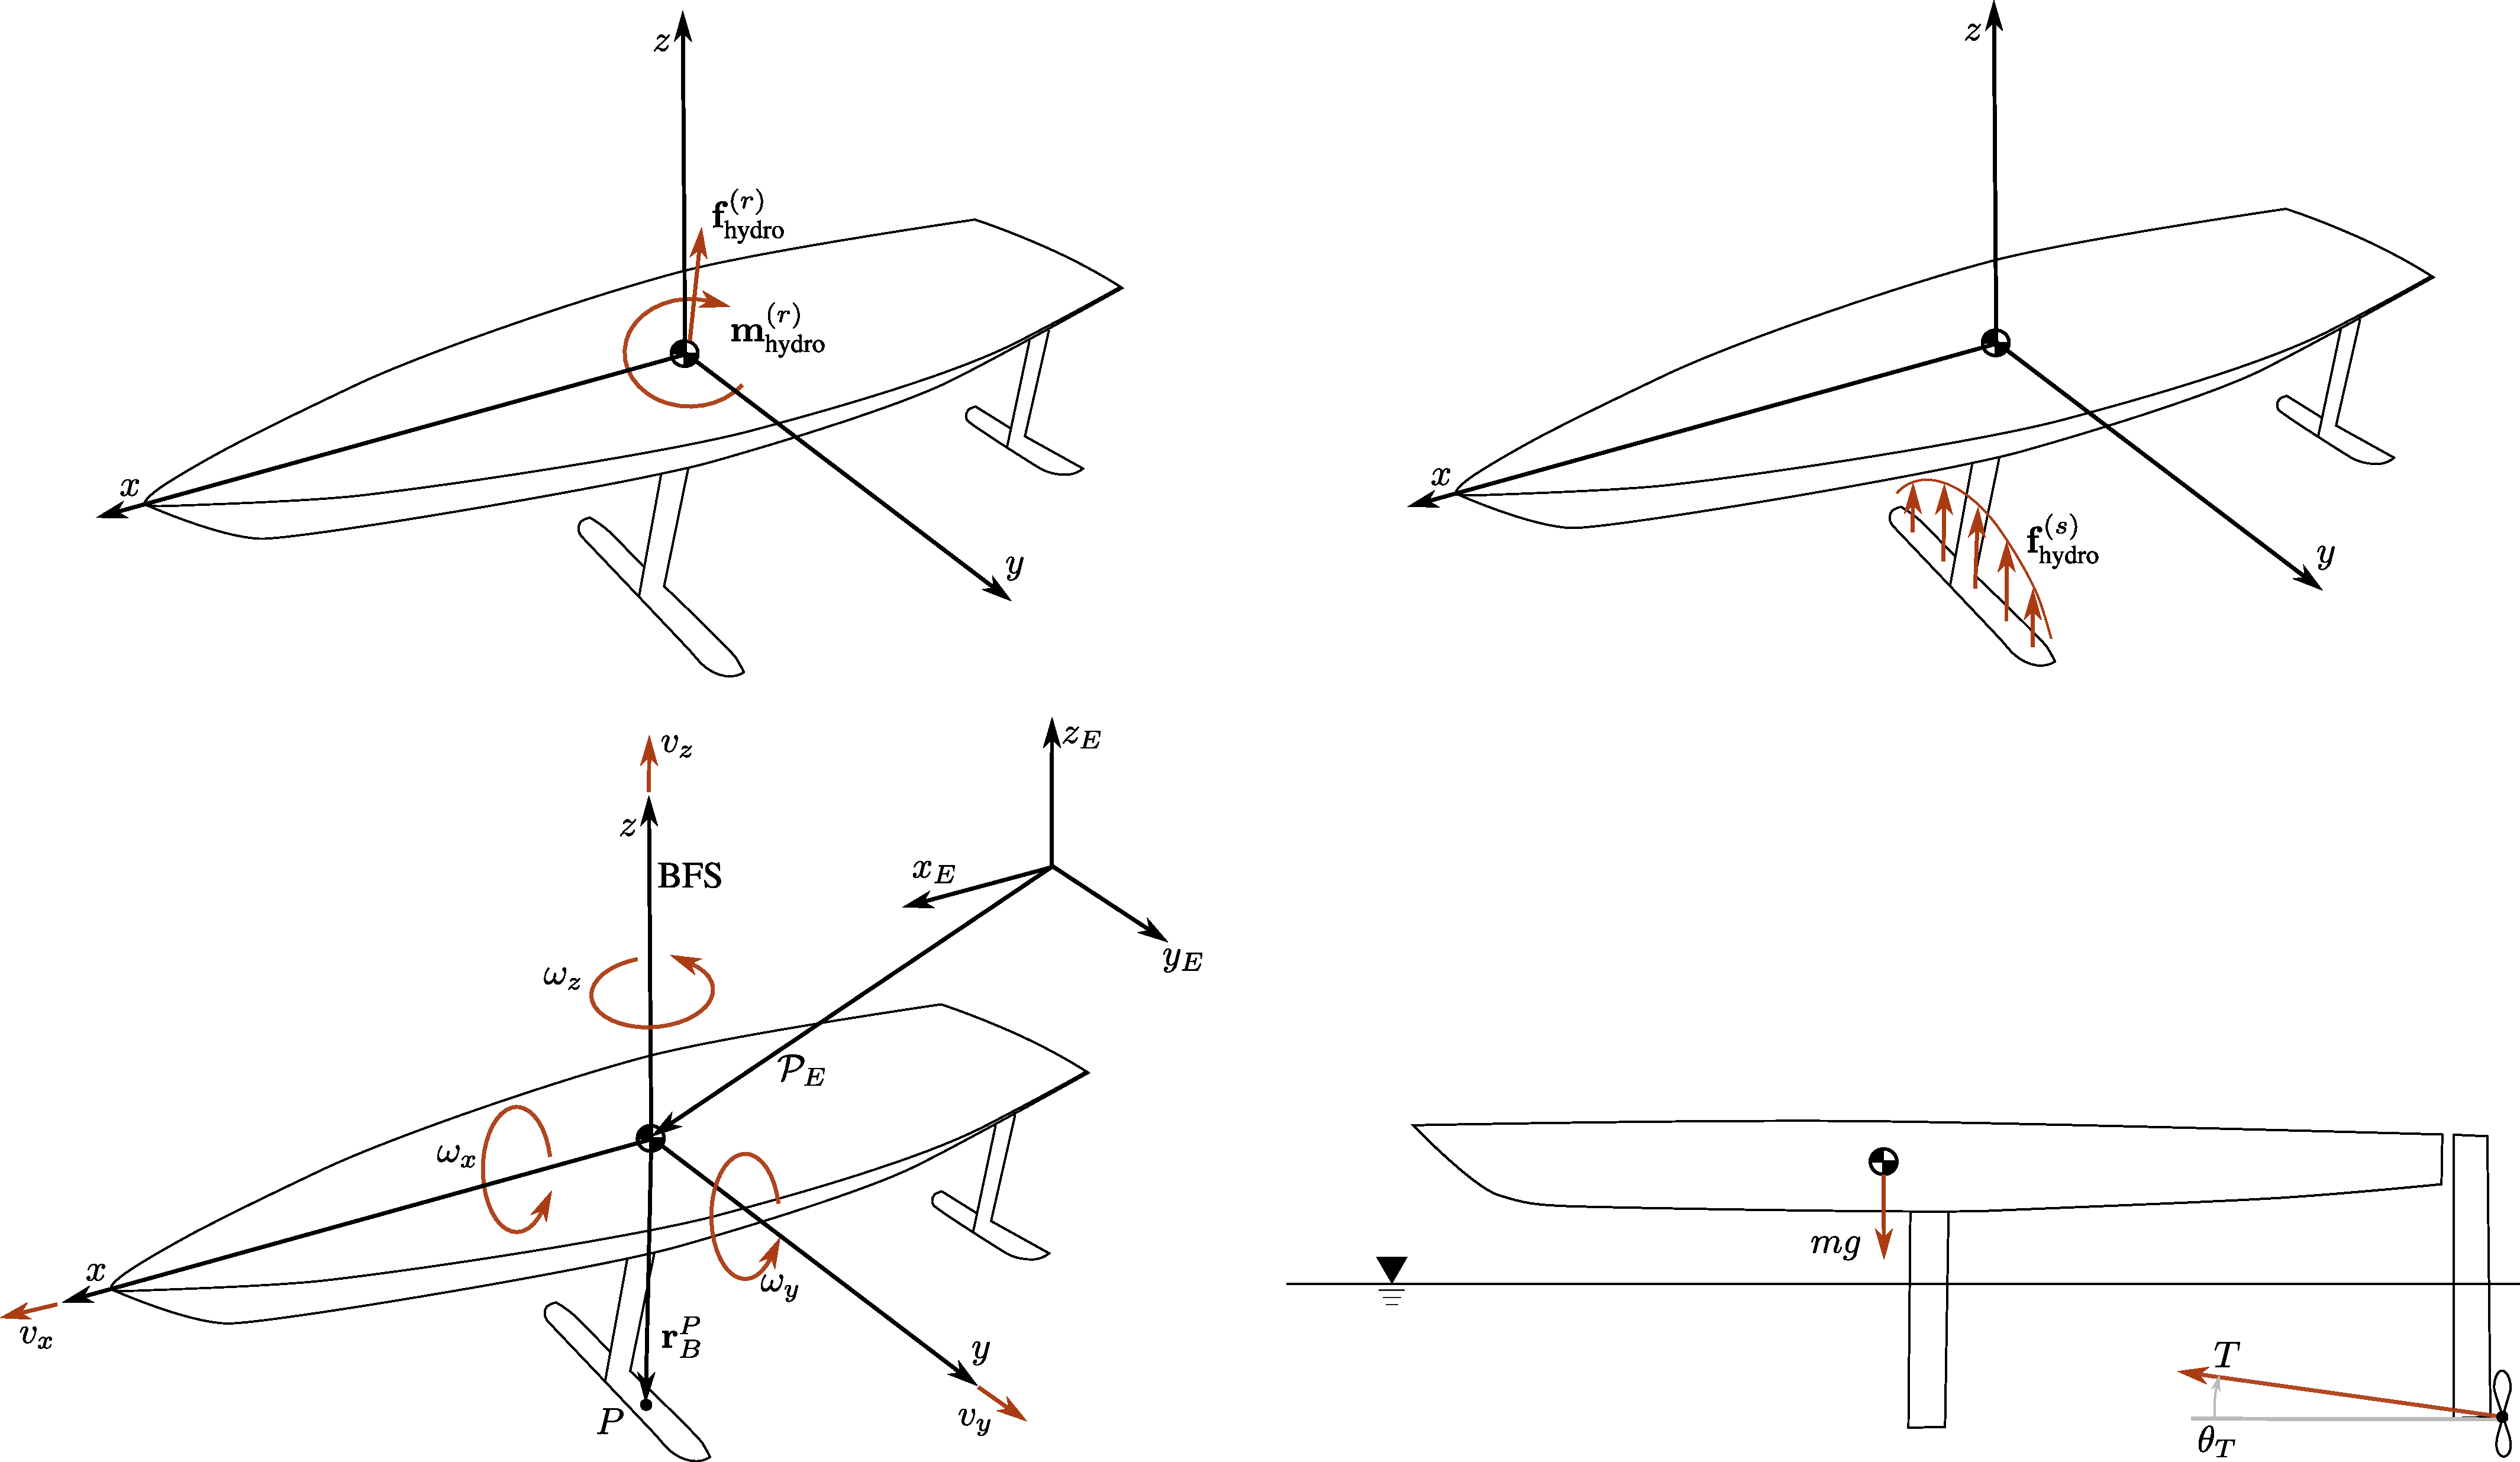
\includegraphics[width=\linewidth,clip,trim={0cm 22cm 0cm 0cm}]{SeakeepingDiagram.pdf}
    \caption{\label{fig:HydroLoads}
        Hydrodynamic loads.
    }
\end{figure*}

\subsection{Steady-state flight solution}
% 
In steady-state flight, there is no acceleration so $\dot{\mbf{v}}_B=\dot{\boldsymbol{\omega}}_B=0$.
Furthermore, $\dot{\phi}=\dot{\theta}=\dot{\psi} = 0, \phi=\theta=0$.
\be
\label{eqn:SteadyState}
\boxed{
    \mbf{f}_{h B} + \mbf{f}_{p B} + \mbf{f}_{g B} - m \tilde{\boldsymbol{\omega}}_B \mbf{v}_B= \mbf{0}
}
\\
\boxed{\mbf{m}_{h B} + \mbf{m}_{p B} - \tilde{\boldsymbol{\omega}}_B \mbf{I}_B \boldsymbol{\omega}_B = \mbf{0}
}
\ee
The pitch of the vessel $\theta$ is treated differently from the trim of the boat $\tau$.
The problem is now finding the $\boldsymbol{\delta}_c$ that satisfy the above equations where the control angles are vessel trim and rudder rake.
\be
\boldsymbol{\delta}_c = \left[
    \tau \quad \delta_r
    \right]^{\top}
\ee
The problem is then solving for the $\boldsymbol{\delta_c}$ that satisfies Equation~\eqref{eqn:SteadyState}.
This can be done with a simple Newton-Raphson root-finding method.

The residual Jacobian needed is
\be
\ee

\subsubsection{Elastified equations of motion}
See \citet[Sec. 5.3.2]{Palacios2023a}.
Defining the state vector as $\mbf{x}_r(t) = [v_x, v_y, v_z, \omega_x, \omega_y, \omega_z, \phi, \theta]^{\top}$ and the control inputs as $\mbf{u} = [\tau, \delta_r]^{\top}$ where $\tau$ and $\delta_r$ are vessel trim and rudder rake command inputs, the dynamics of the system are
\be
\label{eqn:RigidBody}
\dot{\mbf{x}}_r = f^{(r)}(\mbf{x}_r, \mbf{x}_s, \mbf{u}, \mbf{w})
=
f_{\tn{gyr}}^{(r)}\left(\mbf{x}_r\right) + f_{\tn{grav}} \left(\mbf{x}_r\right)
+ f_{\tn{hydro}}^{(r)}\left(\mbf{x}_r, \mbf{x}_s, \mbf{u}\right)
+ f_{\tn{prop}}^{(r)}\left(\mbf{x}_r, \mbf{x}_s, \mbf{u}\right)
\ee
and (under the small amplitude structural deformation assumption) the deformations are determined by
\be
\label{eqn:Struct}
\mbf{K}_{ss} \mbf{x}_s = f^{(s)}\left(\mbf{x}_r, \mbf{x_s}, \mbf{u}\right)
=
f_{\tn{gyr}}^{(s)}\left(\mbf{x}_r\right) + f_{\tn{grav}}\left(\mbf{x}_r\right)
+ f_{\tn{hydro}}^{(s)}\left(\mbf{x}_r, \mbf{x}_s, \mbf{u}\right)
+ f_{\tn{prop}}^{(s)}\left(\mbf{x}_r, \mbf{x}_s, \mbf{u}\right)
\ee
where $\mbf{x}_s(t)$ is the structural state vector.

Equations~\eqref{eqn:RigidBody} and~\eqref{eqn:Struct} are coupled and must be solved simultaneously.
Static trim is $\mbf{x}_{s0}$ and $\mbf{x}_{r0}$.
We solve the coupled system
\beq
& f^{(r)}\left( \mbf{x}_{s0}, \mbf{x}_{r0}, \mbf{u}_{0} \right) & = \mbf{0}
\\
& f^{(s)}\left( \mbf{x}_{s0}, \mbf{x}_{r0}, \mbf{u}_{0} \right)
&=
\mbf{K}_{ss} \mbf{x}_{s0}
\eeq

Assuming small perturbations around the trimmed flight condition, the force Equations~\eqref{eqn:RigidBody} and \eqref{eqn:Struct} can be linearized to
% 
\beq
\label{eqn:CoupledPerturbation}
\Delta \dot{\mbf{x}}_r = \mbf{A}_{rr} \Delta \mbf{x}_r
+ \mbf{A}_{rs} \Delta \mbf{x}_s
+ \mbf{B}_{r} \Delta \mbf{u}
\\
\mbf{K}_{ss} \Delta {\mbf{x}}_s =
\mbf{A}_{sr} \Delta \mbf{x}_r
+ \mbf{A}_{ss} \Delta \mbf{x}_s
+ \mbf{B}_{s} \Delta \mbf{u}
\eeq
% 
where the state ($\mbf{A}$) and input ($\mbf{B}$) matrices are partitions of the Jacobian of nonlinear forcing terms.
This coupled system is linear so we can first solve for
\be
\label{eqn:StructuralPerturbation}
\Delta \mbf{x}_s = \left(\mbf{K}_{ss} - \mbf{A}_{ss}\right)^{-1} \left(\mbf{A}_{sr} \Delta \mbf{x}_r + \mbf{B}_s \Delta \mbf{u} \right)
\ee
and this is substituted back into the first linearized equation in \eqref{eqn:CoupledPerturbation}.
The structural effects are a constant feedback on the rigid equations.
Putting Equation~\eqref{eqn:StructuralPerturbation} into \eqref{eqn:CoupledPerturbation} is called \emph{residualization}.
The implementation in OpenMDAO handles the residualization.

For completeness, the partitions of the Jacobian are
\beq
\mbf{A}_{rr} = \left. \pp{f^{(r)}}{\mbf{x}_r} \right|_{(\mbf{x}_{r0}, \mbf{x}_{s0}, \mbf{u}_0)}
\qquad
\mbf{A}_{ss} = \left. \pp{f^{(s)}}{\mbf{x}_s} \right|_{(\mbf{x}_{r0}, \mbf{x}_{s0}, \mbf{u}_0)}
\\
\mbf{A}_{rs} = \left. \pp{f^{(r)}}{\mbf{x}_s} \right|_{(\mbf{x}_{r0}, \mbf{x}_{s0}, \mbf{u}_0)}
\qquad
\mbf{A}_{sr} = \left. \pp{f^{(s)}}{\mbf{x}_r} \right|_{(\mbf{x}_{r0}, \mbf{x}_{s0}, \mbf{u}_0)}
\\
\mbf{B}_{r} = \left. \pp{f^{(r)}}{\mbf{u}} \right|_{(\mbf{x}_{r0}, \mbf{x}_{s0}, \mbf{u}_0)}
\qquad
\mbf{B}_{s} = \left. \pp{f^{(s)}}{\mbf{u}} \right|_{(\mbf{x}_{r0}, \mbf{x}_{s0}, \mbf{u}_0)}.
\eeq
These must be coded up analytically.

\subsection{Dynamics}
Now in the vibrating mode, if we assume small-amplitude vibrations, we must consider the shift of vehicle center of mass and its impact on the vehicle dynamics.
If the elastic deformations are sufficiently small to not change global inertial characteristics, then modal coordinates can be used.
We introduce a \emph{body-attached frame} (BAF) rigidly linked to a point on the vessel and a \emph{floating frame} (FF).

\section{Data structure and problem setup}

The overall data flow in the program is in \Cref{fig:DataFlow}.
\begin{figure}[htb!]
    \centering
    % reference: trim={<left> <lower> <right> <upper>}
    %   \includesvg[width=\linewidth]{dataFlow.drawio}
    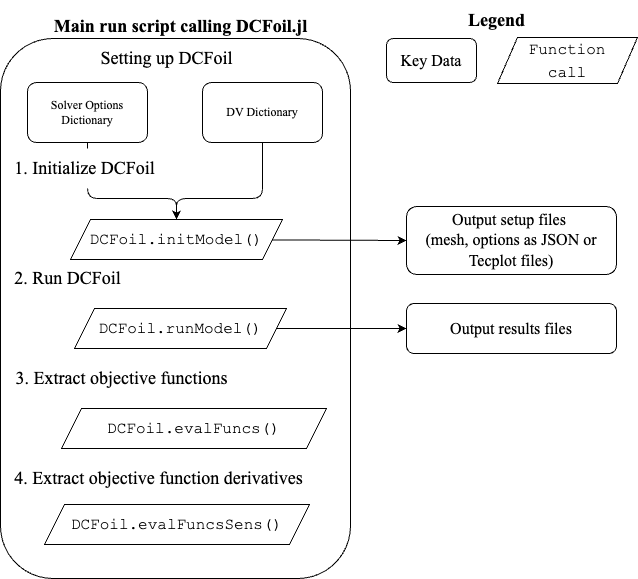
\includegraphics[width=\linewidth,clip,trim={0cm 0cm 0cm 0cm}]{dataFlow.png}
    \caption{\label{fig:DataFlow}Data flow in the program.}
\end{figure}
Appendage setup is through dictionaries.

\section{Writing derivative routines}
% 
The forward and reverse mode AD logic from \citet{Martins2022} is
\ben
\dd{v_i}{v_j} = \dot{v}_i = \sum_{k=j}^{i-1}\pp{v_i}{v_k} \underbrace{\dot{v}_k}_{\dd{v_k}{v_j}}
\\
\dd{v_i}{v_j} = \bar{v}_j = \sum_{k=j+1}^{i}{\pp{v_k}{v_j}} \underbrace{\bar{v}_k}_{\dd{v_i}{v_k}}
\een
where the goal is the LHS (alternative notation $\dd{y}{x}$) over a massive length of code.

The reverse AD routines are in Julia syntax.
Consider the primal function somewhere in the chain of code
\ben
y = f(x)
\een
with a Jacobian matrix $dy/dx$.
The vector-Jacobian product computed by $\mcal{B}$ is
\ben
\pp{a}{x} =
\underbrace{\pp{a}{y}}_{\bar{y}}
\underbrace{\dd{y}{x}}_{\tn{Jacobian }}
= \mcal{B}({\bar{y}})
\een
where $\bar{y}$ is called the \emph{cotangent} vector and $a$ is some known quantity at this stage of the chain rule.
The analog in forward mode are the tangent vector and pushforward function.

The \texttt{pullback} functionality in AD packages typically returns two things: the evaluated point $f(x)$ (also called primal) and the pullback function $\mcal{B}(\bar{y})$
There are situations in which one has a manual implementation they want the {AD} package to bypass, for example, matrix operations.

We write manual rules through \texttt{ChainRules.jl}.
An example is Algorithm~\ref{alg:ConceptualRAD}.
% \usepackage{algorithm2e}
\RestyleAlgo{ruled}
\begin{algorithm}[htb!]
    \caption{\label{alg:ConceptualRAD} Basic reverse rule in Julia ChainRulesCore}
    function ChainRulesCore.rrule(::typeof($f(x)$), $x$)\\
    \quad Evaluate $y = f(x)$ (Primal)\\
    \quad function $\mcal{B}(\bar{y})$\\
    \quad \quad Code up $\bar{x}= \bar{y} \dd{y}{x}$ (Ex. $\cos(x) \bar{y} $ if $f(x)=\sin(x)$)\\
    \quad return $\bar{x}$\\
    return $y$, $\mcal{B}()$
\end{algorithm}

Now that you understand the conceptual level, this is a more applied example for the eigenvalue derivative routine.
\begin{algorithm}[htb!]
    \caption{\label{alg:EigenRAD} Reverse rule for eigenvalue problem}
    function ChainRulesCore.rrule(::typeof(eigvals()), A::AbstractMatrix)\\
    \quad $\lambda_n, \phi_n = \tn{eigvals}(A)$ \\
    return
\end{algorithm}

% \cite{Garg2015,Garg2015a,Garg2016,Garg2017a,Garg2017b,Garg2019a}
% \cite{Liao2019a,Liao2019b,Liao2020a,Liao2020b,Liao2021,Liao2021a,Liao2022,Liao2023}
% \cite{Ng2022a,Ng2022b,Ng2023a}

\onecolumn
\appendix
\bibliography{./gng-link,./mdolab-link}

\end{document}